\documentclass{beamer}

\usetheme{metropolis}

\usepackage{graphicx,xcolor,float}
\usepackage{amssymb,amsmath,array}
\usepackage{setspace,algpseudocode}
\usepackage{wrapfig,caption,subcaption}
\usepackage{chronosys}
\usepackage{multicol}

\usepackage{pgfplots,tikz}
\usetikzlibrary{positioning,arrows}
\pgfplotsset{compat=1.16}

% Black on gray color theme.
\setbeamercolor{frametitle}{fg=white,bg=gray}
\setbeamercolor{title separator}{fg=gray,bg=gray}
\setbeamercolor{normal text}{fg=black,bg=white}
\setbeamercolor{progress bar in head/foot}{fg=black, bg=gray}
\setbeamercolor{progress bar in section page}{ fg=black, bg=gray}

% Table of contents bullet points.
\setbeamertemplate{section in toc}[ball unnumbered]
\setbeamertemplate{subsection in toc}[ball]

% Prevent \maketitle warning caused by bug in the Metropolis theme.
\def\titlepage{%
  \usebeamertemplate{title page}%
}

% Prevent compilation failure caused by Beamer bug.
\makeatletter
\let\@@magyar@captionfix\relax
\makeatother

% Shorten \text command.
\renewcommand{\t}{\text}

\title{Messaging Application with Ratcheting Security}

\date{January 15, 2019}
\author{Andrea Caforio}
\institute{Ecole Polytechnique Fédérale de Lausanne}

\begin{document}
\maketitle

\begin{frame}{Overview}
\tableofcontents
\end{frame}

\section{Ratcheting}
\label{sec:ratcheting}

\begin{frame}{Properties I.}
  \begin{itemize}
  \item Two-party communication protocols.
  \item Key-Agreement or Messaging.
  \item Asynchronous.
  \item Continuous updates of user states (ratchet).
  \end{itemize}
\end{frame}

\begin{frame}{Properties II.}
  \begin{figure}
    \centering
    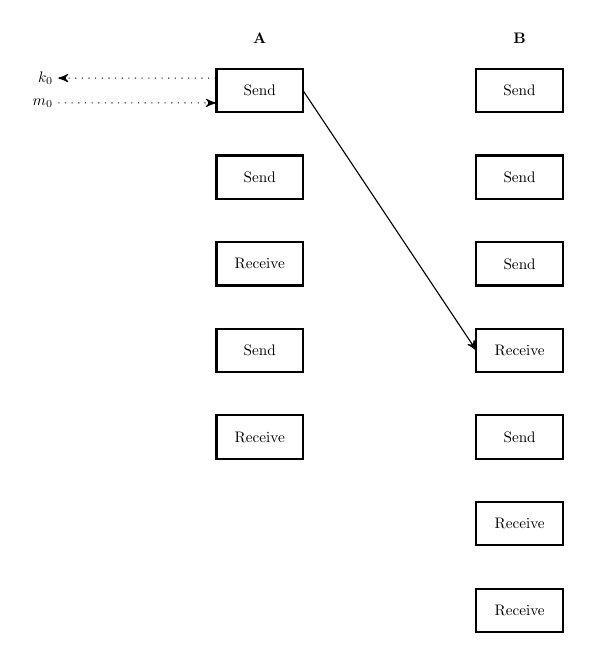
\begin{tikzpicture}[
  box/.style={rectangle,draw,inner sep=5pt,minimum height=1cm,minimum width=2cm,thick},
  node distance=2cm,
  ->,>=stealth',
  scale=0.55, every node/.style={scale=0.55}
]

  % Box t0
  \node [box] (t0) {Send};
  \node [coordinate,right of=t0,node distance=1cm] (tl0) {};
  \node [coordinate,above left=-0.125cm and 0cm of t0,node distance=1cm] (ta0) {};
  \node [left=2cm of ta0] (taa0) {$k_0$};
  \path (ta0) edge[dotted] node [] {} (taa0);
  \node [coordinate,below left=-0.125cm and 0cm of t0,node distance=1cm] (tb0) {};
  \node [left=2cm of tb0] (tbb0) {$m_0$};
  \path (tbb0) edge[dotted] node [] {} (tb0);


  \node [box,below of=t0] (t1) {Send};
  \node [box,below of=t1] (t2) {Receive};
  \node [box,below of=t2] (t3) {Send};
  \node [box,below of=t3] (t4) {Receive};

  \node [box,right of=t0,node distance=6cm] (t5) {Send};
  \node [box,below of=t5] (t6) {Send};
  \node [box,below of=t6] (t7) {Send};
  \node [box,below of=t7] (t8) {Receive};
  \node [box,below of=t8] (t9) {Send};
  \node [box,below of=t9] (t10) {Receive};
  \node [box,below of=t10] (t11) {Receive};

  \node [coordinate,left of=t8,node distance=1cm] (tl8) {};
  \path (tl0) edge[] node [] {} (tl8);

  \node [above=0.25cm of t0] (alice) {\bfseries{A}};
  \node [above=0.25cm of t5] (bob) {\bfseries{B}};
\end{tikzpicture} 
  \end{figure}
\end{frame}

\begin{frame}{Security I.}
  \begin{itemize}
  \item Forward security.
    \begin{itemize}
    \item Protect past states from current state leakages.
    \end{itemize}
  \item Post-compromise security (future secrecy).
    \begin{itemize}
    \item Protect future state from current state leakages.
    \end{itemize}
  \item Assert security through key- or ciphertext-indistinguishability games.
  \end{itemize}
\end{frame}

\begin{frame}{Security II.}
  \begin{figure}[ht]
      \centering
      \setlength{\fboxsep}{10pt}
      \scalebox{0.7}{%
      \fbox{%
         \algrenewcommand\textproc{}
 \algrenewcommand\algorithmicprocedure{\textbf{Game}}

 \begin{minipage}{.5\linewidth}
   \begin{algorithmic}[1]
     \Procedure{$\t{KIND}_b^\mathcal{A}$}{}
     \State $(\t{st}_\t{A},\t{st}_\t{B}) \gets$ \Call{Init}{$1^\lambda$}
     \State $b' \gets \mathcal{A}^{\t{RATCH,EXP,TEST}}$
     \State \Return $b'$
     \EndProcedure
   \end{algorithmic}
 \end{minipage}

 \vline

 \algrenewcommand\textproc{}
 \algrenewcommand\algorithmicprocedure{\textbf{Oracle}}

 \begin{minipage}{.5\linewidth}
   \begin{algorithmic}[1]
     \Procedure{TEST}{$\t{P}$}
     \If{$b = 1$}
     \State \Return $k_\t{P}$
     \EndIf
     \State \Return random $\{0,1\}^{|k_\t{P}|}$ 
     \EndProcedure

     \item[] % Blank line.

     \Procedure{EXP}{$\t{P}$}
     \State \Return $\t{st}_\t{P}$ 
     \EndProcedure
  \end{algorithmic}
\end{minipage}%

      }
    }
  \end{figure}

  \begin{figure}[ht]
      \centering
      \setlength{\fboxsep}{10pt}
      \scalebox{0.7}{%
      \fbox{%
        \algrenewcommand\textproc{}
  \algrenewcommand\algorithmicprocedure{\textbf{Game}}

  \begin{minipage}{.5\linewidth}
    \begin{algorithmic}[1]
      \Procedure{$\t{CIND}_b^\mathcal{A}$}{}
      \State $(\t{st}_\t{A},\t{st}_\t{B}) \gets$ \Call{Init}{$1^\lambda$}
      \State $b' \gets \mathcal{A}^{\t{RATCH',EXP}}$
      \State \Return $b'$
      \EndProcedure
    \end{algorithmic}
  \end{minipage}

  \vline

  \algrenewcommand\textproc{}
  \algrenewcommand\algorithmicprocedure{\textbf{Oracle}}

  \begin{minipage}{.5\linewidth}
    \begin{algorithmic}[1]
      \Procedure{RATCH'}{$\t{P},m_0,m_1$}
      \State \Return \Call{RATCH}{$\t{P},m_b$}
      \EndProcedure

      \item[] % Blank line.

      \Procedure{EXP}{$\t{P}$}
      \State \Return $\t{st}_\t{P}$ 
      \EndProcedure
   \end{algorithmic}
 \end{minipage}%

      }
    }
  \end{figure}
\end{frame}

\begin{frame}{Security III.}
  \begin{itemize}
  \item Powerful adversary.
  \item Many attacks that lead to trivial victories.
  \item Games have to be adapted to exclude these attacks.
  \item The fewer attacks a game disallows the securer the protocol.
  \item Assess advantage of any adversary.
\[
  \t{Adv}(\mathcal{A}) = \left| \Pr \left[ \t{\{C,K\}IND}_0^\mathcal{A} \rightarrow 1 \right] -
                                \Pr \left[ \t{\{C,K\}IND}_1^\mathcal{A} \rightarrow 1 \right]
                         \right|.
\]
  \end{itemize}
\end{frame}

\section{Protocols}
\label{sec:protocols}

\begin{frame}{Timeline I.}
  \begin{enumerate}
  \item \textbf{2012.} Off-the-record messaging protocol.
  \item \textbf{2014.} Signal protocol.
  \item \textbf{2017.} Security analysis of Signal.
  \item \textbf{2017.} Bellare {\em et al.} Formalization of ratcheting. First
    limited, unidirectional protocol.
  \end{enumerate}
\end{frame}

\begin{frame}{Timeline II.}
  \begin{enumerate}
  \item[5.] \textbf{05/2018.} Poettering \& Rösler. Optimally secure bidirectional
    key-agreement protocol (BRKE).
  \item[6.] \textbf{06/2018.} Jager \& Stepanovs. Optimally secure messaging protocol.
  \item[7.] \textbf{09/2018.} Durak \& Vaudenay. Sub-optimally secure, efficient key-agreement
    protocol (BARK).
  \item[8.] \textbf{10/2018.} Jost, Maurer \& Mularczyk. Almost-optimally secure messaging
    protocol.
  \item[9.] \textbf{10/2018.} Alwen, Coretti \& Dodis. Modularization of Signal Double
    Ratchet.
  \end{enumerate}
\end{frame}

\begin{frame}{BRKE (Poettering \& Rösler) I.}
  \begin{itemize}
  \item Optimally secure key-agreement protocol.
    \begin{itemize}
    \item Post-impersonation authenticity.
    \item Post-impersonation confidentiality.
    \end{itemize}
  \item Leverages hierarchical identity-based encryption scheme,
    causing efficiency degradation.
  \end{itemize}
\end{frame}

\begin{frame}{BRKE (Poettering \& Rösler) II.}
  The HIBE is used the mount a key-updatable key encapsulation mechanism (ku-KEM).
  \begin{align*}
    \texttt{Gen} & : \ \rightarrow \mathcal{SK} \times \mathcal{VK} \\
    \texttt{Enc} & : \mathcal{PK} \rightarrow \mathcal{K} \times \mathcal{C} \\ 
    \texttt{Dec} & : \mathcal{SK} \times \mathcal{C} \rightarrow \mathcal{K} \\
    \texttt{UpdPk} & : \mathcal{PK} \times \Delta \rightarrow \mathcal{PK} \\
    \texttt{UpdSk} & : \mathcal{SK} \times \Delta \rightarrow \mathcal{SK}
  \end{align*}
  The protocol further requires a digital signature scheme DS and a random
  oracle H.
\end{frame}

\begin{frame}{BRKE (Poettering \& Rösler) III.}
  \scriptsize
   \begin{minipage}[h]{0.59\textwidth}
      \begin{figure}[h]
        \centering
        \setlength{\fboxsep}{10pt}
        \scalebox{0.7}{%
        \fbox{%
          \algrenewcommand\textproc{}
\algrenewcommand\algorithmicprocedure{\textbf{func}}

\begin{minipage}{1\linewidth}
  {\fontsize{8}{10}\selectfont

  \begin{algorithmic}[1]
    \Procedure{Init}{$K_\t{A},K_\t{B}$}
    \For{$u \in \{A,B\}$}
    \State $(sgk_\t{u},vfk_\t{u}) \gets$ \Call{\texttt{DS.Gen}}{}
    \State $(sk_\t{u},pk_\t{u}) \gets$ \Call{\texttt{ku-KEM.Gen}}{}
    \State $E^\vdash \gets 0, \ E^\dashv \gets 0$
    \State $s \gets 0, \ r \gets 0, \ t \gets \perp$
    \State $PK_\t{u}[0] \gets pk, \ SK_\t{u}[0] \gets sk$
    \State $L_\t{S}[0] \gets \perp, \ L_\t{R}[0] \gets \perp$
    \State $S_\t{u} \gets (PK_{\bar{\t{u}}},E,s,L_\t{S},
                          vfk_{\bar{\t{u}}},K_{\bar{\t{u}}},t)$
    \State $R_\t{u} \gets (SK_\t{u},E,r,L_\t{R},sgk_\t{u},K_\t{u},t)$
    \State $ST_\t{u} \gets (S_\t{u},R_\t{u})$
    \EndFor
    \State \Return $(ST_\t{A},ST_\t{B})$
    \EndProcedure
    
    % \item[]
    
    % \Procedure{Send}{$ST, ad$}
    % \State $(\sigma_\t{root},v,\gamma,T_\t{cur},t_\t{A}) \gets \t{st}_\t{A}$
    % \State $(R,S) \gets ST$
    % \State $(SK,E_\t{R},r,L_\t{R},sgk,K_\t{R},t_\t{R}) \gets R$
    % \State $(sgk^*,vfk^*) \gets$ \Call{\texttt{DS.Gen}}{}
    % \State $(sk^*,pk^*) \gets$ \Call{\texttt{DS.Gen}}{}
    % \State $E_\t{R}^\vdash \gets E_\t{R}^\vdash+1, \ SK[E_\t{R}^\vdash] \gets sk^*$
    % \State $C \gets r || pk^* || vfk^*$
    % \State $(PK,E_\t{S},s,L_\t{S},vfk,K_\t{S},t_\t{S}) \gets S$
    % \State $k^* \gets \perp, \ C \gets C || E_\t{S}^\dashv$
    % \For{$e' \gets E_\t{S}^\vdash$ to $E_\t{S}^\dashv$}
    % \State $(k,c) \gets$ \Call{\texttt{KEM.Enc}}{$PK[e']$}
    % \State $k^* \gets k^* || k, \ C \gets C || c$ 
    % \EndFor
    % \State $\sigma \gets$ \Call{\texttt{DS.Sign}}{$sgk,ad||C$}
    % \State $C \gets C || \sigma, \ L_\t{R}[E_\t{R}^\dashv] \gets ad||C$
    % \State $R \gets (SK,E_\t{R},r,L_\t{R},sgk^*,K_\t{R},t_\t{R})$
    % \State $t_\t{S} \gets ad||C$
    % \State $k.o || K_\t{S} || k.m || sk \gets$ \Call{\texttt{H}}{$K_\t{S},k^*,L_\t{S}$}
    % \State $pk \gets$ \Call{\texttt{ku-KEM.Gen}}{$sk$}
    % \State $PK[...,(E_\t{S}^\dashv -1)] \gets \perp, \ PK[E_\t{S}^\dashv] \gets pk$
    % \State $E_\t{S}^\vdash \gets E_\t{S}^\dashv, \ s \gets s+1, \ L_\t{S}[s] \gets ad||C$
    % \State $S \gets (PK,E_\t{S},s,L_\t{S},vfk,K_\t{S},t_\t{S})$
    % \State $ST \gets (R,S)$
    % \State \Return $(ST,k.o,C)$
    % \EndProcedure
  \end{algorithmic}
  }
\end{minipage}
% \begin{minipage}{0.5\linewidth}
%   {\fontsize{10}{12}\selectfont

%   \begin{algorithmic}[1]
%     \Procedure{Recceive}{$ST,ad,C$}
%     \State $(R,S) \gets ST$
%     \State $(PK,E_\t{S},s,L_\t{S},vfk,K_\t{S},t_\t{S}) \gets S$
%     \State $t^* \gets ad||C, \ t_\t{S} \gets t_\t{S} t^*, \ C || \sigma \gets C$
%     \State \textbf{assert} \Call{\texttt{DS.Verify}}{$vfk,ad||C,\sigma$}
%     \State $r||pk^*||vfk||C \gets C$
%     \State $L\t{S}[...,(r-1)] \gets \perp$
%     \For{$s' \gets r+1$  to $s$}
%     \State $pk^* \gets$ \Call{\texttt{ku-KEM.UpdPk}}{$pk^*,L\t{S}[s']$}
%     \EndFor
%     \State $E_\t{S}^\dashv \gets E_\t{S}^\dashv+1, \ PK[E_\t{S}^\dashv] \gets pk^*$
%     \State $S \gets (PK,E_\t{S},s,L_\t{S},vfk,K_\t{S},t_\t{S})$
%     \State $(SK,E_\t{R},r,L_\t{R},sgk,K_\t{R},t_\t{R}) \gets R$
%     \State $k^* \gets \perp, \ e||C \gets C$
%     \State $t_\t{R} \gets t_\t{R} || L_\t{R}[E_\t{R}^\vdash+1]||...||L_\t{R}[e]$
%     \State $L_\t{R}[...,e] \gets \perp$
%     \For{$e' \gets E_\t{R}^\vdash$ to $e$}
%     \State $c||C \gets C$
%     \State $k \gets$ \Call{\texttt{ku-KEM.Dec}}{$SK[e'],c$}
%     \State $k^* \gets k^* ||k$
%     \EndFor
%     \State $t_\t{R} \gets t_\t{R}||t^*$
%     \State $k.o || K_\t{S} || k.m || sk \gets$ \Call{\texttt{H}}{$K_\t{R},k^*,L_\t{R}$}
%     \State $SK[...,(e -1)] \gets \perp, \ SK[e] \gets sk$
%     \For{$e' \gets e+1$  to $E_\t{R}^\dashv$}
%     \State $SK[e'] \gets$ \Call{\texttt{ku-KEM.UpdSk}}{$SK[e'],t^*$}
%     \EndFor
%     \State $E_\t{R}^\vdash \gets e, \ r \gets r+1$
%     \State $R_\t{u} \gets (SK_\t{u},E,r,L_\t{R},sgk_\t{u},K_\t{u},t)$
%     \State $ST \gets (R,S)$
%     \State \Return $(ST,k.o)$ 
%     \EndProcedure
%   \end{algorithmic}
%   }
% \end{minipage}
        }
      }
    \end{figure}
    \end{minipage}
   \begin{minipage}[h]{0.40\textwidth}
      \begin{itemize}
      \item $E^\vdash,E^\dashv$: Epoch counters.
      \item $s, r$: Sent and received counters.
      \item $t, L_S, L_R$: Transcript accumulators.
      \end{itemize}
  \end{minipage}
\end{frame}

\begin{frame}{BRKE (Poettering and Rösler) IV.}
  \scriptsize
  \begin{figure}[h]
        \centering
        \setlength{\fboxsep}{10pt}
        \scalebox{0.6}{%
        \fbox{%
          \algrenewcommand\textproc{}
\algrenewcommand\algorithmicprocedure{\textbf{func}}

\begin{minipage}{1\linewidth}
  {\fontsize{8}{10}\selectfont

  \begin{algorithmic}[1]
    \Procedure{Send}{$ST, ad$}
    \State $(\sigma_\t{root},v,\gamma,T_\t{cur},t_\t{A}) \gets \t{st}_\t{A}$
    \State $(R,S) \gets ST$
    \State $(SK,E_\t{R},r,L_\t{R},sgk,K_\t{R},t_\t{R}) \gets R$
    \State $(sgk^*,vfk^*) \gets$ \Call{\texttt{DS.Gen}}{}
    \State $(sk^*,pk^*) \gets$ \Call{\texttt{DS.Gen}}{}
    \State $E_\t{R}^\vdash \gets E_\t{R}^\vdash+1, \ SK[E_\t{R}^\vdash] \gets sk^*$
    \State $C \gets r || pk^* || vfk^*$
    \State $(PK,E_\t{S},s,L_\t{S},vfk,K_\t{S},t_\t{S}) \gets S$
    \State $k^* \gets \perp, \ C \gets C || E_\t{S}^\dashv$
    \For{$e' \gets E_\t{S}^\vdash$ to $E_\t{S}^\dashv$}
    \State $(k,c) \gets$ \Call{\texttt{KEM.Enc}}{$PK[e']$}
    \State $k^* \gets k^* || k, \ C \gets C || c$ 
    \EndFor
    \State $\sigma \gets$ \Call{\texttt{DS.Sign}}{$sgk,ad||C$}
    \State $C \gets C || \sigma, \ L_\t{R}[E_\t{R}^\dashv] \gets ad||C$
    \State $R \gets (SK,E_\t{R},r,L_\t{R},sgk^*,K_\t{R},t_\t{R})$
    \State $t_\t{S} \gets ad||C$
    \State $k.o || K_\t{S} || k.m || sk \gets$ \Call{\texttt{H}}{$K_\t{S},k^*,L_\t{S}$}
    \State $pk \gets$ \Call{\texttt{ku-KEM.Gen}}{$sk$}
    \State $PK[...,(E_\t{S}^\dashv -1)] \gets \perp, \ PK[E_\t{S}^\dashv] \gets pk$
    \State $E_\t{S}^\vdash \gets E_\t{S}^\dashv, \ s \gets s+1, \ L_\t{S}[s] \gets ad||C$
    \State $S \gets (PK,E_\t{S},s,L_\t{S},vfk,K_\t{S},t_\t{S})$
    \State $ST \gets (R,S)$
    \State \Return $(ST,k.o,C)$
    \EndProcedure
  \end{algorithmic}
  }
\end{minipage}

        }
      }
    \end{figure}
       \begin{itemize}
       \item Transcript is accumulated.
       \item Key-updates only for deferred messages.
       \item All keys are used in the encapsulation when the direction changes.
       \end{itemize}
\end{frame}

\begin{frame}{BRKE (Poettering and Rösler) V.}
  \scriptsize
    \begin{figure}[h]
        \centering
        \setlength{\fboxsep}{10pt}
        \scalebox{0.6}{%
        \fbox{%
          \algrenewcommand\textproc{}
\algrenewcommand\algorithmicprocedure{\textbf{func}}

\begin{minipage}{1.2\linewidth}
  {\fontsize{8}{10}\selectfont
    \begin{multicols}{2}
  \begin{algorithmic}[1]
    \Procedure{Receive}{$ST,ad,C$}
    \State $(R,S) \gets ST$
    \State $(PK,E_\t{S},s,L_\t{S},vfk,K_\t{S},t_\t{S}) \gets S$
    \State $t^* \gets ad||C, \ t_\t{S} \gets t_\t{S} t^*, \ C || \sigma \gets C$
    \State \textbf{assert} \Call{\texttt{DS.Verify}}{$vfk,ad||C,\sigma$}
    \State $r||pk^*||vfk||C \gets C$
    \State $L\t{S}[...,(r-1)] \gets \perp$
    \For{$s' \gets r+1$  to $s$}
    \State $pk^* \gets$ \Call{\texttt{ku-KEM.UpdPk}}{$pk^*,L\t{S}[s']$}
    \EndFor
    \State $E_\t{S}^\dashv \gets E_\t{S}^\dashv+1, \ PK[E_\t{S}^\dashv] \gets pk^*$
    \State $S \gets (PK,E_\t{S},s,L_\t{S},vfk,K_\t{S},t_\t{S})$
    \State $(SK,E_\t{R},r,L_\t{R},sgk,K_\t{R},t_\t{R}) \gets R$
    \State $k^* \gets \perp, \ e||C \gets C$
    \State $t_\t{R} \gets t_\t{R} || L_\t{R}[E_\t{R}^\vdash+1]||...||L_\t{R}[e]$
    \State $L_\t{R}[...,e] \gets \perp$
    \For{$e' \gets E_\t{R}^\vdash$ to $e$}
    \State $c||C \gets C$
    \State $k \gets$ \Call{\texttt{ku-KEM.Dec}}{$SK[e'],c$}
    \State $k^* \gets k^* ||k$
    \EndFor
    \State $t_\t{R} \gets t_\t{R}||t^*$
    \State $k.o || K_\t{S} || k.m || sk \gets$ \Call{\texttt{H}}{$K_\t{R},k^*,L_\t{R}$}
    \State $SK[...,(e -1)] \gets \perp, \ SK[e] \gets sk$
    \For{$e' \gets e+1$  to $E_\t{R}^\dashv$}
    \State $SK[e'] \gets$ \Call{\texttt{ku-KEM.UpdSk}}{$SK[e'],t^*$}
    \EndFor
    \State $E_\t{R}^\vdash \gets e, \ r \gets r+1$
    \State $R_\t{u} \gets (SK_\t{u},E,r,L_\t{R},sgk_\t{u},K_\t{u},t)$
    \State $ST \gets (R,S)$
    \State \Return $(ST,k.o)$ 
    \EndProcedure
  \end{algorithmic}
  \end{multicols}
  }
\end{minipage}
        }
      }
   \end{figure}
       \begin{itemize}
       \item Key-updates for deferred messages.
       \item Communication transcript is accumulated.
       \item The more encapsulations the bigger the ciphertext.
       \end{itemize}
\end{frame}

\begin{frame}{Secure Channel (Jaeger and Stepanovs) I.}
  \begin{itemize}
  \item Optimally secure messaging protocol.
  \item Also uses HIBE scheme to provide provide key-update
    functionalities.
  \end{itemize}
\end{frame}

\begin{frame}{Secure Channel (Jaeger and Stepanovs) II.}
  The HIBE is used to build a key-updatable public-key encryption scheme (ku-PKE).
  \begin{align*}
    \texttt{Gen} & : \ \rightarrow \mathcal{DK} \times \mathcal{EK} \\
    \texttt{Enc} & : \mathcal{EK} \times \mathcal{M} \rightarrow \mathcal{C} \\
    \texttt{Dec} & : \mathcal{DK} \times \mathcal{C} \rightarrow \mathcal{M} \\
    \texttt{UpdEk} & : \mathcal{EK} \times \Delta \rightarrow \mathcal{EK} \\
    \texttt{UpdDk} & : \mathcal{DK} \times \Delta \rightarrow \mathcal{DK}
  \end{align*}
\end{frame}

\begin{frame}{Secure Channel (Jaeger and Stepanovs) III.}
  It further needs a key-updatable digital signature scheme (ku-DS).
  \begin{align*}
    \texttt{Gen} & \  \rightarrow \mathcal{SK} \times \mathcal{VK} \\
    \texttt{Sign} & : \mathcal{SK} \times \mathcal{M} \rightarrow \Sigma \\
    \texttt{Verify} & : \mathcal{VK} \times \mathcal{M} \times \Sigma \rightarrow \{0,1\} \\
    \texttt{UpdSk} & : \mathcal{SK} \times \Delta \rightarrow \mathcal{SK} \\
    \texttt{UpdVk} & : \mathcal{VK} \times \Delta \rightarrow \mathcal{VK}
  \end{align*}
  Unlike the ku-PKE the ku-DS is mounted by forward-secure signature scheme.
  We also need a collision-resistant hash function H.
\end{frame}

\begin{frame}{Secure Channel (Jaeger and Stepanovs) IV.}
  \scriptsize
  \begin{minipage}[h]{0.65\textwidth}
      \begin{figure}[h]
        \centering
        \setlength{\fboxsep}{10pt}
        \scalebox{0.7}{%
        \fbox{%
          \algrenewcommand\textproc{}
\algrenewcommand\algorithmicprocedure{\textbf{func}}

\begin{minipage}{1\linewidth}
  {\fontsize{8}{10}\selectfont

  \begin{algorithmic}[1]
    \Procedure{Init}{}
    \State $(sk_\t{I},vk_\t{R}) \gets \texttt{ku-DS.Gen}$
    \State $(ek_\t{I},dk_\t{R}[0]) \gets \texttt{ku-PKE.Gen}$
    \State $(sk_\t{R},vk_\t{I}) \gets \texttt{ku-DS.Gen}$
    \State $(ek_\t{R},dk_\t{I}[0]) \gets \texttt{ku-PKE.Gen}$
    \State $st_\t{I} \gets \t{H.Gen}, \ T_\t{R} \gets [\cdot], \ T_\t{S}[0] \gets \perp$
    \State $s \gets 0, \ r \gets 0, \ r^\t{ack} \gets 0$
    \State $st_\t{I} \gets (s,r,r^\t{ack},sk_\t{I},vk_\t{I},ek_\t{I},dk_\t{I},hk,T_\t{R},T_\t{S})$
    \State $st_\t{R} \gets (s,r,r^\t{ack},sk_\t{R},vk_\t{R},ek_\t{R},dk_\t{R},hk,T_\t{R},T_\t{S})$
    \EndProcedure
  \end{algorithmic}
  }
\end{minipage}
        }
      }
    \end{figure}
    \end{minipage}
  \begin{minipage}[h]{0.34\textwidth}
      \begin{itemize}
      \item $s, r$: Sent and receive counters.
      \item $r^\t{ack}$: Number of acknowledged messages.
      \item $T_S,T_R$: Message transcript arrays.
      \end{itemize}
    \end{minipage}
\end{frame}

\begin{frame}{Secure Channel (Jaeger and Stepanovs) V.}
  \scriptsize
  \begin{minipage}[ht]{0.59\textwidth}
      \begin{figure}[ht]
        \centering
        \setlength{\fboxsep}{10pt}
        \scalebox{0.7}{%
        \fbox{%
          \algrenewcommand\textproc{}
\algrenewcommand\algorithmicprocedure{\textbf{func}}

\begin{minipage}{1\linewidth}
  {\fontsize{8}{10}\selectfont
  \begin{algorithmic}[1]
    \Procedure{Send}{$st, ad,m$}
    \State $(s,r,r^\t{ack},sk,vk,ek,dk,hk,T_\t{R},T_\t{S}) \gets st$
    \State $s \gets s+1$
    \State $(sk',vk') \gets \texttt{ku-DS.Gen}$
    \State $(ek',dk[s]) \gets \texttt{ku-PKE.Gen}$
    \State $l \gets (s,r,ad,vk',ek',T_\t{R},T_\t{S}[s-1])$
    \State $ek' \gets ek$
    \For{$i \gets r^\t{ack}+1$ to $s$}
    \State $ek' \gets$ \Call{\texttt{ku-PKE.UpdEk}}{$ek', T_\t{S}[i]$}
    \EndFor
    \State $c' \gets$ \Call{\texttt{ku-PKE.Enc}}{$ek',l,m,T_\t{S}$}
    \State $v \gets (c',l), \ \sigma \gets \texttt{ku-DS.Sign}(sk,v)$
    \State $c \gets (\sigma,v), \ T_\t{S}[s] \gets \texttt{H}(hk,c)$
    \State $st \gets (s,r,r^\t{ack},sk',vk,ek,dk,hk,T_\t{R},T_\t{S})$
    \State \Return $(st,c)$
    \EndProcedure
  \end{algorithmic}
  }
\end{minipage}

        }
      }
    \end{figure}
    \end{minipage}
  \begin{minipage}[ht]{0.40\textwidth}
      \begin{itemize}
      \item 1 ku-PKE generation for the reply, 1 ku.DS generation for the next message.
      \item Unidirectional traffic has quadratic ku-PKE key-update penalty.
      \item Entire receive transcript is part of message.
      \end{itemize}
    \end{minipage}
\end{frame}

\begin{frame}{Secure Channel (Jaeger and Stepanovs) VI.}
  \scriptsize
  \begin{minipage}[h]{0.65\textwidth}
      \begin{figure}[ht]
        \centering
        \setlength{\fboxsep}{10pt}
        \scalebox{0.7}{%
        \fbox{%
          \algrenewcommand\textproc{}
\algrenewcommand\algorithmicprocedure{\textbf{func}}

\begin{minipage}{1\linewidth}
  {\fontsize{8}{10}\selectfont
  \begin{algorithmic}[1]
    \Procedure{Receive}{$st,ad,c$}
    \State $(s,r,r^\t{ack},sk,vk,ek,dk,hk,T_\t{R},T_\t{S}) \gets st$
    \State $(\sigma,v) \gets c, \ (c',l) \gets v$
    \State $(s',r',ad',vk',ek',T_\t{R}',T_\t{S}') \gets l$
    \State $vk'' \gets vk$
    \For{$i \gets r^\t{ack}+1$ to r'}
    \State $vk'' \gets$ \Call{\texttt{ku-DS.UpdVk}}{$vk'', T_\t{S}[i]$}
    \EndFor
    \State \textbf{assert} \Call{\texttt{ku-DS.Verify}}{$vk'',\sigma,v,T_\t{S}$}
    \State $r \gets r+1, \ r^\t{ack} \gets r'$
    \State $m \gets \texttt{ku-PKE.Dec}(dk[r^\t{ack}],l,c')$
    \State $T_\t{S}[...,r^\t{ack}] \gets \perp, \ dk_\t{S}[...,r^\t{ack}] \gets \perp$
    \State $T_\t{R} \gets \texttt{H}(hk,c), \ sk \gets \texttt{ku-DS.UpdSk}(sk,T_\t{R})$
    \For{$i = r^\t{ack}$ to $s$}
    \State $dk[i] \gets$ \Call{\texttt{ku-PKE.UpdDk}}{$dk[i],T_\t{R}$}
    \EndFor
    \State $st \gets (s,r,r^\t{ack},sk,vk',ek',dk,hk,T_\t{R},T_\t{S})$
    \State \Return $(st,m)$
    \EndProcedure
  \end{algorithmic}
  }
\end{minipage}
        }
      }
    \end{figure}
    \end{minipage}
  \begin{minipage}[h]{0.34\textwidth}
      \begin{itemize}
      \item ku-DS signing key updated with each receive. Incurs
        linearly many verification key-updates when direction changes.
      \end{itemize}
    \end{minipage}
\end{frame}

\begin{frame}{BARK (Durak \& Vaudenay) I.}
  \begin{itemize}
  \item Sub-optimally secure but very efficient key-agreement protocol.
  \item Relies only on regular public-key cryptosystems.
  \item Recover security.
  \item Composed of a simpler unidirectional messaging protocol (uniARCAD),
    one instance per user.
  \end{itemize}
\end{frame}

\begin{frame}{BARK (Durak \& Vaudenay) II.}
  BARK relies on a simple signcryption construction, combining a public-key
  encryption scheme and digital signature scheme.
  \begin{align*}
    \texttt{PKE.Gen} & : \ \rightarrow \mathcal{SK}_\t{R} \times \mathcal{PK}_\t{R} \\
    \texttt{DS.Gen} & : \ \rightarrow \mathcal{SK}_\t{S} \times \mathcal{PK}_\t{S} \\
    \texttt{Enc} & : \mathcal{SK}_\t{S} \times \mathcal{PK}_\t{R} \times \mathcal{M} \times
                   \mathcal{AD} \rightarrow \mathcal{C} \\
    \texttt{Dec} & : \mathcal{SK}_\t{R} \times \mathcal{PK}_\t{S} \times
  \mathcal{C} \times \mathcal{AD} \rightarrow \mathcal{M}
  \end{align*}
  It further needs some collision-resistant hash function H.
\end{frame}

\begin{frame}{BARK (Durak \& Vaudenay) III.}
   \begin{figure}[h]
     \centering
     \setlength{\fboxsep}{10pt}
     \scalebox{0.7}{%
       \fbox{%
          \algrenewcommand\textproc{}
\algrenewcommand\algorithmicprocedure{\textbf{func}}

\begin{minipage}{.5\linewidth}
  {\fontsize{8}{10}\selectfont

    \begin{algorithmic}[1]
    \Procedure{Init}{}
    \State $(sk_\t{S},pk_\t{S}) \gets$ \Call{\texttt{PKE.Gen}}{}
    \State $(sk_\t{R},pk_\t{R}) \gets$ \Call{\texttt{DS.Gen}}{}

    \State $st_\t{S} \gets (sk_S,pk_\t{R})$ 
    \State $st_\t{R} \gets (sk_R,pk_\t{S})$ 

    \State \Return $(st_\t{S},st_\t{R})$
    \EndProcedure
    \end{algorithmic}

    \vspace{10pt}

    \begin{algorithmic}[1]
    \Procedure{Receive}{$st_\t{R}, ad, ct$}
    \State $(sk_\t{R},pk_\t{S}) \gets st_\t{R}$ 
    \State $pt' \gets$ \Call{\texttt{Dec}}{$sk_\t{R},pk_\t{S},ad,ct$}
    \If{$pt' = \perp$}
    \State \Return $(\t{false}, st_\t{R}, \perp)$
    \EndIf
    \State $(pt,st_\t{R}') \gets pt'$
    \State \Return $(\t{true},st_\t{R}, pt)$
    \EndProcedure
   
  \end{algorithmic}
  }
\end{minipage}

\begin{minipage}{.5\linewidth}
  {\fontsize{8}{10}\selectfont

  \begin{algorithmic}[1]
    \Procedure{Send}{$st_\t{S}, ad, pt, \t{flag}$}
    \State $(sk_\t{S},pk_\t{R}) \gets st_\t{S}$ 
    \If{$\t{flag} = \t{true}$}
    \State $(sk_\t{S}',pk_\t{S}') \gets$ \Call{\texttt{PKE.Gen}}{}
    \State $(\t{sk}_\t{R}',\t{pk}_\t{R}') \gets$ \Call{\texttt{DS.Gen}}{}
    \State $st_\t{S}' \gets (sk_\t{S}',pk_\t{R}')$
    \State $st_\t{R}' \gets (sk_\t{R}',pk_\t{S}')$
    \Else
    \State $(sk_\t{S}',pk_\t{R}') \gets (\perp,\perp)$
    \EndIf
    \State $pt' \gets st_\t{R}' || pt$
    \State $ct \gets$ \Call{\texttt{Enc}}{$sk_\t{S},pk_\t{R}, ad, pt'$}
    \State \Return $(st_\t{S}', ct)$
    \EndProcedure
    
  \end{algorithmic}
  }
\end{minipage}

       }
     }
  \end{figure}
\end{frame}

\begin{frame}{BARK (Durak \& Vaudenay) IV.}
   \scriptsize
  \begin{minipage}[h]{0.49\textwidth}
      \begin{figure}[ht]
        \centering
        \setlength{\fboxsep}{10pt}
        \scalebox{0.7}{%
        \fbox{%
          \algrenewcommand\textproc{}
\algrenewcommand\algorithmicprocedure{\textbf{func}}

\begin{minipage}{\linewidth}
  {\fontsize{8}{10}\selectfont
  \begin{algorithmic}[1]
    \Procedure{Init}{}
    \State $(st_\t{A}^\t{send},st_\t{B}^\t{rec}) \gets$ \Call{\texttt{uniBARK.Init}}{}
    \State $(st_\t{B}^\t{send},st_\t{A}^\t{rec}) \gets$ \Call{\texttt{uniBARK.Init}}{}
    \State pick $hk$ at random
    \State $st_\t{A} \gets (hk, [st_\t{A}^\t{send}], [st_\t{A}^\t{rec}],\perp,\perp)$ 
    \State $st_\t{B} \gets (hk, [st_\t{B}^\t{send}], [st_\t{B}^\t{rec}],\perp,\perp)$ 
    \State \Return $(st_\t{A},st_\t{B})$
    \EndProcedure
  \end{algorithmic}
  }
\end{minipage}

        }
      }
    \end{figure}
    \end{minipage}
  \begin{minipage}[h]{0.49\textwidth}
      \begin{itemize}
      \item Initialize two uniARCAD instances and distribute the
        resulting states.
      \item Further initialize two variables (Hsent, Hreceived) to $\perp$ which will
        hold the chain-hash of all sent and received messages.
      \end{itemize}
    \end{minipage}
  \end{frame}

\begin{frame}{BARK (Durak \& Vaudenay) V.}
  \scriptsize
  \begin{figure}[ht]
     \centering
     \setlength{\fboxsep}{10pt}
     \scalebox{0.5}{%
       \fbox{%
         \algrenewcommand\textproc{}
\algrenewcommand\algorithmicprocedure{\textbf{func}}

\begin{minipage}{\linewidth}
  {\fontsize{8}{10}\selectfont
  \begin{algorithmic}[1]
    \Procedure{Send}{$st_\t{P}$}
    \State pick $k$ at random
    \State $(hk, [st_\t{P}^\t{send,1},...,st_\t{P}^\t{send,u}],
                 [st_\t{P}^\t{rec,1},...,st_\t{P}^\t{rec,v}],
    \t{Hsent}, \t{Hreceived}) \gets st_\t{P}$
    \State $(st_\t{S,new},st_\t{P}^\t{rec,v+1}) \gets$ \Call{\texttt{uniARCAD.Init}}{}
    \State $\t{onion} \gets st_\t{S,new} || k$
    \State find smallest i such that $st_\t{P}^\t{send,i} \neq \perp$
    \For{$j \gets u$ to $i$}
    \State $(st_\t{P}^\t{send,j},\t{onion}) \gets$ \Call{\texttt{uniARCAD.Send}}
               {$st_\t{P}^\t{send,j},(u-j)||\t{onion},j=u$}
    \If{$j < u$}
    \State $st_\t{P}^\t{send,j} \gets \perp$
    \EndIf
    \EndFor

    \State $\t{upd} \gets (u-i)||\t{Hsent}||\t{onion}$
    \State $\t{Hsent}' \gets$ \Call{\texttt{H}}{hk,\t{upd}}
    \State $st_\t{P}' \gets (hk,[st_\t{P}^\t{send,1},...,st_\t{P}^\t{send,u}],
                 [st_\t{P}^\t{rec,1},...,st_\t{P}^\t{rec,v+1}], \t{Hsent}', \t{Hreceived})$

    \State \Return $(st_\t{P}', \t{upd})$
    \EndProcedure
  \end{algorithmic}
  }
\end{minipage}

       }
     }
  \end{figure}
  \begin{itemize}
  \item Create 2 new uniARCAD instances, 1 one for the next message and 1
    for the reply.
  \item Accumulate uniARCAD states and use all in onion encryption when
    the direction changes.
  \end{itemize}
\end{frame}

\begin{frame}{BARK (Durak \& Vaudenay) VI.}
  \scriptsize
  \begin{figure}[ht]
     \centering
     \setlength{\fboxsep}{10pt}
     \scalebox{0.5}{%
       \fbox{%
         \algrenewcommand\textproc{}
\algrenewcommand\algorithmicprocedure{\textbf{func}}

\begin{minipage}{\linewidth}
  {\fontsize{8}{10}\selectfont
  \begin{algorithmic}[1]
    \Procedure{Receive}{$st_\t{P}, \t{upd}$}
    \State $(hk, [st_\t{P}^\t{send,1},...,st_\t{P}^\t{send,u}],
                 [st_\t{P}^\t{rec,1},...,st_\t{P}^\t{rec,v}],
    \t{Hsent}, \t{Hreceived}) \gets st_\t{P}$
    \State $(n,h,\t{onion}) \gets \t{upd}$
    \If{$h \neq \t{Hreceived}$}
    \State \Return $(\t{false},st_\t{P},\perp)$
    \EndIf
    \State find smallest i such that $st_\t{P}^\t{rec,i} \neq \perp$
    \For{$j \gets i$ to $i+n$}
    \State $(\t{acc},st_\t{P}^\t{rec,j'},\t{onion}) \gets$ \Call{\texttt{uniARCAD.Receive}}
    {$st_\t{P}^\t{rec,j}$}
    \If{$\t{acc} = \t{false}$}
    \State \Return $(\t{false},st_\t{P},\perp)$
    \EndIf
    \EndFor

    \State $(st_\t{P}^\t{send,u+1},k) \gets \t{onion}$
    \For{$j \gets i$ to $i+n-1$}
    \State $st_\t{P}^\t{rec,j} \gets \perp$
    \EndFor
    \State $st_\t{P}^\t{rec,i+n} \gets st_\t{P}^\t{rec,i+n'}$
    \State $\t{Hreceived}' \gets$ \Call{\texttt{H}}{$hk,\t{upd}$}
    \State $st_\t{P}' \gets (hk,[st_\t{P}^\t{send,1},...,st_\t{P}^\t{send,u+1}],
                 [st_\t{P}^\t{rec,1},...,st_\t{P}^\t{rec,v}], \t{Hsent}, \t{Hreceived}')$

    \State \Return $(\t{true}, st_\t{P}',k)$
    \EndProcedure
  \end{algorithmic}
  }
\end{minipage}

       }
     }
  \end{figure}
  \begin{itemize}
  \item Chain-hash the communication transcript to ensure recover security.
  \end{itemize}
\end{frame}

\begin{frame}{Secure Channel (Jost, Maurer \& Mularczyk) I.}
  \begin{itemize}
  \item Aims to fill the gap between BARK and the first two protocols.
  \item Almost completely post-impersonation secure but less efficient than BARK.
  \item As BARK only relies on regular public-key cryptosystems however
    it proposes several rather complicated key-update primitives.
  \end{itemize}
\end{frame}

\begin{frame}{Secure Channel (Jost, Maurer \& Mularczyk) II.}
  The first primitive is a key-updatable signature scheme (ku-Sig).
  \begin{align*}
    \texttt{Gen} & : \ \rightarrow \mathcal{VK} \times \mathcal{SK} \\
    \texttt{Sign} & : \mathcal{SK} \times \mathcal{M} \rightarrow \mathcal{SK} \times \Sigma \\
    \texttt{Verify} & : \mathcal{VK} \times \mathcal{M} \times \Sigma
             \rightarrow \mathcal{VK} \times \{0,1\}
  \end{align*}
A ku-Sig can be constructed out of a regular digital signature scheme.
\end{frame}

\begin{frame}{Secure Channel (Jost, Maurer \& Mularczyk) III.}
  The protocol further needs a secretly key-updatable public-key encryption scheme (sku-PKE).
   \begin{align*}
     \texttt{Gen} & : \ \rightarrow \mathcal{EK} \times \mathcal{DK}, \
     && \texttt{UpdGen} : \ \rightarrow \mathcal{UE} \times \mathcal{UD} \\
     \texttt{Enc} & : \mathcal{EK} \times \mathcal{M} \rightarrow \mathcal{C}, \
     && \texttt{UpdEk} : \mathcal{UE} \times \mathcal{EK} \rightarrow \mathcal{EK} \\
     \texttt{Dec} & : \mathcal{DK} \times \mathcal{C} \rightarrow \mathcal{M}, \
     && \texttt{UpdDk} :  \mathcal{UD} \times \mathcal{DK} \rightarrow \mathcal{DK}
  \end{align*}
The update information is independently generated and the keys
can be separately updated. A sku-PKE can be mounted with the
components of the ElGamal cryptosystem.
\end{frame}

\begin{frame}{Secure Channel (Jost, Maurer \& Mularczyk) IV.}
  The sku-PKE serves as a building block a healable and key-updating
  public-key encryption scheme (hku-PKE). We further need a regular
  PKE that can treat associated data (PKE-AD).
  \begin{align*}
    \texttt{Gen} & : \ \rightarrow \mathcal{EK} \times \mathcal{DK}, \ &&
    \texttt{BcUpEk} : \mathcal{EK} \times \Delta \rightarrow \mathcal{EK} \\
    \texttt{Enc} & : \mathcal{EK} \times \mathcal{M} \times \mathcal{AD}
                   \rightarrow \mathcal{C}, \ &&
    \texttt{BcUpDk} : \mathcal{DK} \times \Delta \rightarrow \mathcal{DK} \\
    \texttt{Dec} & : \mathcal{DK} \times \mathcal{C} \times \mathcal{AD}
                   \rightarrow \mathcal{M}
  \end{align*}
  Update calls do not to be synchronized anymore, meaning that decryption still
  succeeds for any sequence of \texttt{BcUpDk} call even if only a prefix
  of the used update information has been used in \texttt{BcUpEk} calls.
\end{frame}

\begin{frame}{Secure Channel (Jost, Maurer \& Mularczyk) V.}
  \scriptsize
  \begin{figure}[ht]
     \centering
     \setlength{\fboxsep}{10pt}
     \scalebox{0.6}{%
       \fbox{%
         \algrenewcommand\textproc{}
\algrenewcommand\algorithmicprocedure{\textbf{func}}
\begin{minipage}{\linewidth}
  {\fontsize{10}{12}\selectfont
  \begin{algorithmic}[1]
    \Procedure{Init}{}
    \For{$u \in \{A,B\}$}
      \State $(ek_u,dk_u) \gets$ \Call{\texttt{hku-PKE.Gen}}{}
      \State $(sk_u^\t{upd},vk_u^\t{upd}) \gets$ \Call{\texttt{ku-Sig.Gen}}{}
      \State $(sk_u^\t{eph},vk_u^\t{eph}) \gets$ \Call{\texttt{Sig.Gen}}{}
    \EndFor
    \For{$u \in \{A,B\}$}
    \State $st_u \gets (0,0,0,dk_u,ek_{\bar{u}},sk_u^\t{upd},vk_{\bar{u}}^\t{upd},
                        sk_u^\t{eph},vk_{\bar{u}}^\t{ep},[\cdot],\perp,[\cdot])$
    \EndFor
    \State \Return $(st_\t{A},st_\t{B})$
    \EndProcedure
   \end{algorithmic}
  }
\end{minipage}

       }
     }
  \end{figure}
  \begin{itemize}
  \item Protocol also needs a regular digital signature scheme (Sig).
  \item Set sent and receive counters $(s,r)$ as well number of acknowledged
    messages $s_\t{ack}$ to 0.
  \item Further initialize a Sig verification key array $VK^\t{eph}$, a transcript
    variable holding the chain-hash of the messages $tr$ and a transcript array $TR$.
  \end{itemize}
\end{frame}

\begin{frame}{Secure Channel (Jost, Maurer \& Mularczyk) VI.}
  \scriptsize
  \begin{figure}[ht]
     \centering
     \setlength{\fboxsep}{10pt}
     \scalebox{0.6}{%
       \fbox{%
         \algrenewcommand\textproc{}
\algrenewcommand\algorithmicprocedure{\textbf{func}}
\begin{minipage}{\linewidth}
  {\fontsize{10}{12}\selectfont
  \begin{algorithmic}[1]
    \Procedure{Send}{$st,m$}
    \State $(r,s,s_\t{ack},dk,ek,sk^\t{upd},vk^\t{upd},
                        sk^\t{eph},vk^\t{eph},VK^\t{eph},tr,TR) \gets st$
    \State $(sk_1^\t{eph},vk_1^\t{eph}) \gets$ \Call{\texttt{Sig.Gen}}{}
    \State $(sk_2^\t{eph},vk_2^\t{eph}) \gets$ \Call{\texttt{Sig.Gen}}{}

    \State $(dk,upd) \gets$ \Call{\texttt{hku-PKE.BcUpDk}}{$dk$}
    \State $c \gets$ \Call{\texttt{hku-PKE.Enc}}{$ek,m||sk_1^\t{eph},upd||vk_2^\t{eph}||r$}
    \State $c' \gets c||upd||vk_2^\t{eph}||r$
    \State $(sk^\t{upd},\sigma_\t{upd}) \gets$ \Call{\texttt{ku-Sig.Sign}}{$sk^\t{upd},c'||tr$}
    \State $\sigma_\t{eph} \gets$ \Call{\texttt{Sig.Sign}}{$sk^\t{eph},c'||tr$}

    \State $s \gets s+1$
    \State $VK[s] \gets vk_1^\t{eph}$
    \State $TR[s] \gets$ \Call{\texttt{H}}{$Tr[s-1]||c'$}
    
    
    \State $st \gets (r,s,s_\t{ack},dk,ek,sk^\t{upd},vk^\t{upd},
                        sk_2^\t{eph},vk^\t{ep},VK^\t{eph},tr,TR)$
    
    \State \Return $(st, (c',\sigma_\t{upd},\sigma_\t{eph}))$
    \EndProcedure
   \end{algorithmic}
  }
\end{minipage}

       }
     }
  \end{figure}
  \begin{itemize}
  \item Generate two sets of Sig key pairs for sending and receiving and
    accumulate the verification key.
  \item Update hku-PKE keys for each message.
  \item Combination of ku-Sig and Sig signature yields post-impersonation
    authenticity.
  \end{itemize}
\end{frame}

\begin{frame}{Secure Channel (Jost, Maurer \& Mularczyk) VII.}
  \scriptsize
  \begin{figure}[ht]
     \centering
     \setlength{\fboxsep}{10pt}
     \scalebox{0.55}{%
       \fbox{%
         \algrenewcommand\textproc{}
\algrenewcommand\algorithmicprocedure{\textbf{func}}
\begin{minipage}{\linewidth}
  {\fontsize{10}{12}\selectfont
  \begin{algorithmic}[1]
    \Procedure{Receive}{$st,ct$}
    \State $(r,s,s_\t{ack},dk,ek,sk^\t{upd},vk^\t{upd},
                        sk^\t{eph},vk^\t{eph},VK^\t{eph},tr,TR) \gets st$
    \State $(c',\sigma_\t{upd},\sigma_\t{eph}) \gets ct$
    \State $(c,upd,vk_\t{msg}^\t{eph},s_\t{msg}) \gets c'$
    \If{$s_\t{msg} > s_\t{ack}$}
    \State $vk \gets VK^\t{eph}[s_\t{msg}]$
    \Else
    \State $vk \gets vk^\t{eph}$
    \EndIf

    \State $v_\t{eph} \gets$
    \Call{\texttt{Sig.Verify}}{$vk,c'||TR[s_\t{msg}],\sigma_\t{eph}$}
    \State $(vk^\t{upd},v_\t{upd}) \gets$
    \Call{\texttt{ku-Sig.Verify}}{$vk^\t{upd},c', \sigma_\t{upd}$}
    \State \textbf{assert} $v_\t{eph} \wedge v_\t{upd}$

    \State $ek \gets$ \Call{\texttt{hku-PKE.BcUpEk}}{$ek,upd$} 
    \State $(dk, (m,sk_\t{msg}^\t{eph})) \gets$
    \Call{\texttt{hku-PKE.Dec}}{$dk,c,upd||vk_\t{msg}^\t{eph}||s_\t{msg}$}
    \State $r \gets r +1$
    \State $tr \gets$ \Call{\texttt{H}}{$tr||c'$}
    
    \State $st \gets (r,s,s_\t{msg},dk,ek,sk^\t{upd},vk^\t{upd},
                        sk_\t{msg}^\t{eph},vk_\t{msg}^\t{ep},VK^\t{eph},tr,TR)$

    \State \Return $(st,m)$
    \EndProcedure
  \end{algorithmic}
  }
\end{minipage}

       }
     }
  \end{figure}
  \begin{itemize}
  \item Message transcript is accumulated.
  \item Use accumulated verification keys if $s_\t{msg} > s_\t{ack}$ otherwise
    use received verification keys.
  \end{itemize}
\end{frame}

\begin{frame}{Double Ratchet (Alwen, Coretti \& Dodis) I.}
  \begin{itemize}
  \item Attempt to formalize and modularize Signal's double ratchet protocol.
  \item Unlike the other protocols, it uses private-key cryptography to ensure
    forward-secrecy hence it does not reach the same security guarantees.
  \item However, this approach yields a very efficient protocol.
  \item Only protocol that offers immediate decryption.
  \end{itemize}
\end{frame}

\begin{frame}{Double Ratchet (Alwen, Coretti \& Dodis) II.}
  A forward-secure authenticated encryption scheme with associated data (FS-AEAD)
  provides forward security.
  \begin{align*}
    \t{FS-Init-S} & : \mathcal{K} \rightarrow \mathcal{V}_S \\
    \t{FS-Init-R} & : \mathcal{K} \rightarrow \mathcal{V}_R \\
    \t{FS-Send} & : \mathcal{V}_S \times \mathcal{AD} \times \mathcal{M}
                                \rightarrow \mathcal{V}_S \times \mathcal{C} \\
    \t{FS-Rcv} & : \mathcal{V}_R \times \mathcal{AD} \times \mathcal{C}
                                \rightarrow \mathcal{V}_R \times \mathcal{C}.
  \end{align*}
  A FS-AEAD can be mounted with AES-GCM.
\end{frame}

\begin{frame}{Double Ratchet (Alwen, Coretti \& Dodis) III.}
  As in the Signal protocol there is a key-agreement protocol for periodically
  renegotiating symmetric keys, called continuous key-agreement (CKA).
  \begin{align*}
    \texttt{CKA-Init-S} & : \mathcal{K} \rightarrow \mathcal{V}_A \\
    \texttt{CKA-Init-R} & : \mathcal{K} \rightarrow \mathcal{V}_B \\
    \texttt{CKA-S} & : \mathcal{V}_A \rightarrow
                \mathcal{V}_A \times \mathcal{T} \times \mathcal{I} \\
    \texttt{CKA-R} & : \mathcal{V}_B \times \mathcal{T} \rightarrow
                \mathcal{V}_B \times \mathcal{I}.
  \end{align*}
  The CKA is synchronized, meaning that the parties take turns instigating
  key-agreements. It can be constructed out of a generic KEM based on
  the decisional Diffie-Hellman assumption.
\end{frame}

\begin{frame}{Double Ratchet (Alwen, Coretti \& Dodis) IV.}
  Finally, to generate the same randomness for both participants a stateful
  blend between a PRF and PRNG is constructed.
  \begin{align*}
    \t{P-Init} & : \mathcal{K} \rightarrow \Sigma \\
    \t{P-Up} & : \Sigma \times \mathcal{I} \rightarrow \Sigma \times \mathcal{I}.
  \end{align*}
  A PRF-PRNG can be instantiated with a HKDF.
\end{frame}

\begin{frame}{Double Ratchet (Alwen, Coretti \& Dodis) V.}
  \scriptsize
   \begin{minipage}[h]{0.49\textwidth}
      \begin{figure}[h]
        \centering
        \setlength{\fboxsep}{10pt}
        \scalebox{0.7}{%
        \fbox{%
          \algrenewcommand\textproc{}
\algrenewcommand\algorithmicprocedure{\textbf{func}}

\begin{minipage}{1\linewidth}
  {\fontsize{8}{10}\selectfont

  \begin{algorithmic}[1]
    \Procedure{Init-A}{$k$}
    \State $(k_\t{root},k_\t{CKA}) \gets k$
    \State $\sigma_\t{root} \gets$ \Call{\texttt{P-Init}}{$k_\t{root}$}
    \State $v \gets []$
    \State $(\sigma_\t{root},k) \gets$ \Call{\texttt{P-Up}}{$\sigma_\t{root},\perp$}
    \State $v[0] \gets$ \Call{\texttt{FS-Init-R}}{$k$}
    \State $\gamma \gets$ \Call{\texttt{CKA-Init-A}}{$k_\t{CKA}$}
    \State $T_\t{cur} \gets \perp, \ t_\t{A} \gets 0$
    \State $st_\t{A} \gets (\sigma_\t{root},v,\gamma,T_\t{cur},t_\t{A})$
    \State \Return $st_\t{A}$
    \EndProcedure
  \end{algorithmic}
  }
\end{minipage}

        }
      }
    \end{figure}
    \end{minipage}
   \begin{minipage}[h]{0.49\textwidth}
      \begin{itemize}
      \item $\sigma_\t{root}$: PRF-PRNG state.
      \item $\gamma$: CKA state.
      \item $T_\t{cur}$: CKA update information.
      \item $t_\t{P}$: Epoch counter.
      \end{itemize}
  \end{minipage}
\end{frame}

\begin{frame}{Double Ratchet (Alwen, Coretti \& Dodis) VI.}
  \scriptsize
   \begin{minipage}[h]{0.49\textwidth}
      \begin{figure}[h]
        \centering
        \setlength{\fboxsep}{10pt}
        \scalebox{0.7}{%
        \fbox{%
          \algrenewcommand\textproc{}
\algrenewcommand\algorithmicprocedure{\textbf{func}}

\begin{minipage}{1\linewidth}
  {\fontsize{8}{10}\selectfont

  \begin{algorithmic}[1]
    \Procedure{Send-A}{$st_\t{A}, m$}
    \State $(\sigma_\t{root},v,\gamma,T_\t{cur},t_\t{A}) \gets st_\t{A}$
    \If{$t_\t{A}$ is even}
    \State $v[t_\t{A}-1] \gets \perp$
    \State $t_\t{A} \gets t_\t{A}+1$
    \State $(\gamma,T_\t{cur},I) \gets$ \Call{\texttt{CKA-S}}{$\gamma$}
    \State $(\sigma_\t{root},k) \gets$ \Call{\texttt{P-Up}}{$\sigma_\t{root},I$}
    \State $v[t_\t{A}] \gets$ \Call{\texttt{FS-Init-S}}{$k$}
    \EndIf
    \State $h \gets (t_\t{A},T_\t{cur})$
    \State $(v[t_\t{A}],e) \gets$ \Call{\texttt{FS-Send}}{$v[t_\t{A}],h,m$}
    \State $c \gets (h,e)$
    \State \Return $(st_\t{A},c)$
    \EndProcedure
  \end{algorithmic}
  }
\end{minipage}
        }
      }
    \end{figure}
    \end{minipage}
   \begin{minipage}[h]{0.49\textwidth}
      \begin{itemize}
      \item CKA output used to generate FS-AEAD key via PRF-PRNG.
      \item As in Signal CKA is renegotiated at the start of every epoch.
      \end{itemize}
  \end{minipage}
\end{frame}

\begin{frame}{Double Ratchet (Alwen, Coretti \& Dodis) VII.}
  \scriptsize
   \begin{minipage}[h]{0.49\textwidth}
      \begin{figure}[h]
        \centering
        \setlength{\fboxsep}{10pt}
        \scalebox{0.7}{%
        \fbox{%
          \algrenewcommand\textproc{}
\algrenewcommand\algorithmicprocedure{\textbf{func}}

\begin{minipage}{1\linewidth}
  {\fontsize{8}{10}\selectfont

  \begin{algorithmic}[1]
    \Procedure{Rcv-A}{$st_\t{A},c$}
    \State $(\sigma_\t{root},v,\gamma,T_\t{cur},t_\t{A}) \gets st_\t{A}$
    \State $(h,e) \gets c, \ (t,T) \gets h$
    \If{$t \leq t_\t{A}$ and even}
    \State $(v[t],i,m) \gets$ \Call{\texttt{FS-Rcv}}{$v[t],h,e$}
    \ElsIf{$t = t_\t{A}+1$ and $t_\t{A}$ odd}
    \State $t_\t{A} \gets t_\t{A}+1$
    \State $v[t-2] \gets \perp$
    \State $\gamma,I) \gets$ \Call{\texttt{CKA-R}}{$\gamma,T$}
    \State $(\sigma_\t{root},k) \gets$ \Call{\texttt{P-Up}}{$\sigma_\t{root},I$}
    \State $(v[t]) \gets$ \Call{\texttt{FS-Init-R}}{$k$}
    \State $(v[t],i,m) \gets$ \Call{\texttt{FS-Rcv}}{$v[t],h,e$}
    \EndIf
    \State \Return $(st_\t{A},t,i,m)$
    \EndProcedure
  \end{algorithmic}
  }
\end{minipage}

        }
      }
    \end{figure}
    \end{minipage}
   \begin{minipage}[h]{0.49\textwidth}
      \begin{itemize}
      \item State size only grows in case of message reorder or message-loss.
      \end{itemize}
  \end{minipage}
\end{frame}

\section{Benchmarks}
\label{sec:benchmarks}

\begin{frame}{Incentive}
  \begin{itemize}
  \item Solidify performance differences.
  \item Gain insight into the feasibility of a potential real-world usage.
  \item Spot performance weakness that can be tackled in updated protocol
    versions.
  \end{itemize}
\end{frame}

\begin{frame}{Setup I.}
  \begin{itemize}
  \item Implementation in Go (all protocols \& some primitives).
    \begin{itemize}
    \item Compiled and garbage-collected (disabled for benchmarks).
      Efficiency close to C/C++.
    \item Built-in industry-grade benchmark tooling.
    \end{itemize}
  \item Intel Core i5 with 8GB RAM (comparable to high-end smartphone).
  \end{itemize}
\end{frame}

\begin{frame}{Setup II.}
  \begin{itemize}
  \item \textbf{Runtime.} How long it takes to exchange $n$ messages
    executed on a single machine ignoring potential latency that would occur in a network.
  \item \textbf{Message Size.} The maximal size of a messages throughout the
    exchange of $n$ messages. A message designates the data that is sent over the channel.
  \item \textbf{State Size.} The maximal size of a user state throughout the
    exchange of $n$ messages. The state designates all the data kept in memory by a user.
  \end{itemize}
\end{frame}

\begin{frame}{Setup III.}
  \begin{itemize}
  \item \textbf{Alternating.} Alice and Bob take turns sending messages.
    Alice sends the odd- numbered messages and Bob sends the even-numbered messages.
  \item \textbf{Unidirectional.} Alice first sends $\frac{n}{2}$ messages to Bob,
    after receiving them Bob responds with the remaining $\frac{n}{2}$ messages.
  \item \textbf{Deferred Unidirectional.} Alice first sends $\frac{n}{2}$ messages
    to Bob but before he receives them, Bob sends his share of $\frac{n}{2}$ messages to Alice.
  \end{itemize}
\end{frame}

\begin{frame}{Setup IV.}
  \begin{figure}[H]
    \centering
    \noindent\begin{subfigure}[t]{0.32\linewidth}
      \centering
      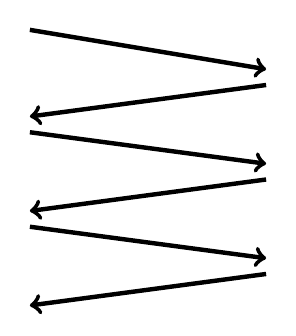
\begin{tikzpicture}

  % Message 1
  \node [coordinate] (a1) {};
  \node [coordinate,below right=0.5cm and 3cm of a1] (b1) {};
  \draw [->,ultra thick] (a1) -- node [above,midway] {} (b1);

  % Message 2
  \node [coordinate,below=0.2cm of b1] (b2) {};
  \node [coordinate,below left=0.4cm and 3cm of b2] (a2) {};
  \draw [->,ultra thick] (b2) -- node [above,midway] {} (a2);

  % Message 3
  \node [coordinate,below=0.2cm of a2] (a3) {};
  \node [coordinate,below right=0.4cm and 3cm of a3] (b3) {};
  \draw [->,ultra thick] (a3) -- node [above,midway] {} (b3);

  % Message 4
  \node [coordinate,below=0.2cm of b3] (b4) {};
  \node [coordinate,below left=0.4cm and 3cm of b4] (a4) {};
  \draw [->,ultra thick] (b4) -- node [above,midway] {} (a4);

  % Message 5
  \node [coordinate,below=0.2cm of a4] (a5) {};
  \node [coordinate,below right=0.4cm and 3cm of a5] (b5) {};
  \draw [->,ultra thick] (a5) -- node [above,midway] {} (b5);

  % Message 6
  \node [coordinate,below=0.2cm of b5] (b6) {};
  \node [coordinate,below left=0.4cm and 3cm of b6] (a6) {};
  \draw [->,ultra thick] (b6) -- node [above,midway] {} (a6);

\end{tikzpicture}
      \caption{Alternating}
    \end{subfigure}%
    \begin{subfigure}[t]{0.32\linewidth}
      \centering
      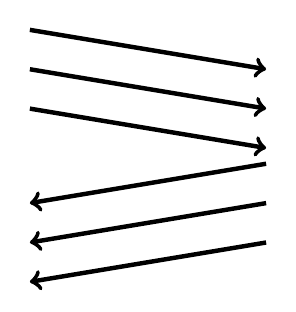
\begin{tikzpicture}

  % Message 1
  \node [coordinate] (a1) {};
  \node [coordinate,below right=0.5cm and 3cm of a1] (b1) {};
  \draw [->,ultra thick] (a1) -- node [above,midway] {} (b1);

  % Message 2
  \node [coordinate,below=0.5cm of a1] (a2) {};
  \node [coordinate,below right=0.5cm and 3cm of a2] (b2) {};
  \draw [->,ultra thick] (a2) -- node [above,midway] {} (b2);

  % Message 3
  \node [coordinate,below=0.5cm of a2] (a3) {};
  \node [coordinate,below right=0.5cm and 3cm of a3] (b3) {};
  \draw [->,ultra thick] (a3) -- node [above,midway] {} (b3);

  % Message 4
  \node [coordinate,below=0.2cm of b3] (b4) {};
  \node [coordinate,below left=0.5cm and 3cm of b4] (a4) {};
  \draw [->,ultra thick] (b4) -- node [above,midway] {} (a4);

  % Message 5
  \node [coordinate,below=0.5cm of b4] (b5) {};
  \node [coordinate,below left=0.5cm and 3cm of b5] (a5) {};
  \draw [->,ultra thick] (b5) -- node [above,midway] {} (a5);

  % Message 6
  \node [coordinate,below=0.5cm of b5] (b6) {};
  \node [coordinate,below left=0.5cm and 3cm of b6] (a6) {};
  \draw [->,ultra thick] (b6) -- node [above,midway] {} (a6);

\end{tikzpicture}
      \caption{Unidirectional}
    \end{subfigure}%
    \begin{subfigure}[t]{0.32\linewidth}
      \centering
      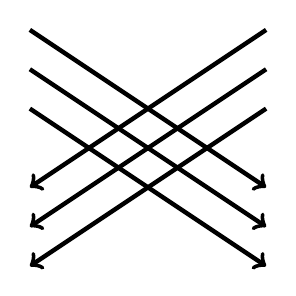
\begin{tikzpicture}

  % Message 1
  \node [coordinate] (a1) {};
  \node [coordinate,below right=2cm and 3cm of a1] (b1) {};
  \draw [->,ultra thick] (a1) -- node [above,midway] {} (b1);

  % Message 2
  \node [coordinate,below=0.5cm of a1] (a2) {};
  \node [coordinate,below right=2cm and 3cm of a2] (b2) {};
  \draw [->,ultra thick] (a2) -- node [above,midway] {} (b2);

  % Message 3
  \node [coordinate,below=0.5cm of a2] (a3) {};
  \node [coordinate,below right=2cm and 3cm of a3] (b3) {};
  \draw [->,ultra thick] (a3) -- node [above,midway] {} (b3);

  % Message 4
  \node [coordinate,right=3cm of a1] (b4) {};
  \node [coordinate,below left=2cm and 3cm of b4] (a4) {};
  \draw [->,ultra thick] (b4) -- node [above,midway] {} (a4);

  % Message 5
  \node [coordinate,below=0.5cm of b4] (b5) {};
  \node [coordinate,below left=2cm and 3cm of b5] (a5) {};
  \draw [->,ultra thick] (b5) -- node [above,midway] {} (a5);

  % Message 6
  \node [coordinate,below=0.5cm of b5] (b6) {};
  \node [coordinate,below left=2cm and 3cm of b6] (a6) {};
  \draw [->,ultra thick] (b6) -- node [above,midway] {} (a6);

\end{tikzpicture}
      \caption{Def. Unidirectional}
    \end{subfigure}
  \end{figure}
\end{frame}

\begin{frame}{Primitives I.}
  \begin{itemize}
  \item \textbf{SHA-256.} As the hash function and random oracle. Part of
    the Go standard library.
  \item \textbf{AES-GCM.} As the AEAD scheme (e.g. in FS-AEAD). Part of
    the Go standard library.
  \item \textbf{Gentry-Silverberg HIBE.} As the HIBE scheme in the first
    two protocols. Implemented by hand.
  \end{itemize}
\end{frame}

\begin{frame}{Primitives II.}
  \begin{itemize}
   \item \textbf{ECIES.} As the public-key encryption scheme in several protocols.
    Implemented by hand.
  \item \textbf{ECDSA.} As the digital signature scheme in several protocols.
    Part of the Go standard library.
  \item \textbf{Bellare et al. Forward-Secure Signature} As the forward-secures
    signature within the ku-DSS. Implemented by hand.
  \end{itemize}
\end{frame}

\begin{frame}{Runtime (Alternating) I.}
  \begin{figure}[H]
    \centering
    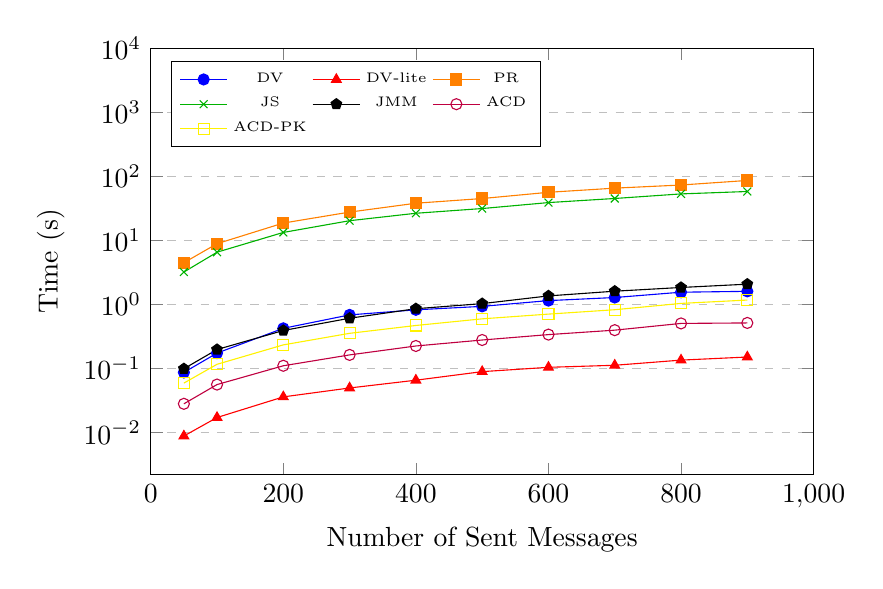
\begin{tikzpicture}[scale=1]
\begin{axis}[
  %title=Alternating,
  ymode=log,
  legend style={font=\tiny, legend columns=3},
  scaled ticks=false,
  xlabel={Number of Sent Messages},
  ylabel={Time (s)},
  xmin=0, xmax=1000,
  ymax=10000,
  xtick={0,200,400,600,800,1000},
  ytick={0.01,0.1,1,10,100,1000,10000},
  legend pos=north west,
  ymajorgrids=true,
  xminorticks=false,
  yminorticks=false,
  grid style=dashed,
  height=7cm,
  width=10cm,
]
 
\addplot[color=blue,mark=*]
   coordinates {
  (50,0.0874)(100,0.175)(200,0.426)(300,0.690)(400,0.828)(500,0.938)(600,1.153)
  (700,1.288)(800,1.559)(900,1.609)
  };

\addplot[color=red,mark=triangle*]
  coordinates {
  (50,0.0089)(100,0.0173)(200,0.0363)(300,0.0500)(400,0.0661)(500,0.0899)
  (600,0.105)(700,0.113)(800,0.136)(900,0.152)
  };

\addplot[color=orange,mark=square*]
  coordinates {
  (50,4.5)(100,8.9)(200,18.7)(300,27.7)(400,38.1)(500,45.1)
  (600,56.4)(700,65.5)(800,73.3)(900,86.3)
  };

\addplot[color=black!30!green,mark=x]
  coordinates {
  (50,3.217)(100,6.560)(200,13.343)(300,20.338)(400,26.564)(500,31.485)
  (600,38.999)(700,45.183)(800,53.249)(900,58.065)
  };

\addplot[color=black,mark=pentagon*]
  coordinates {
  (50,0.0998)(100,0.199)(200,0.394)(300,0.612)(400,0.862)(500,1.035)
  (600,1.365)(700,1.617)(800,1.848)(900,2.081)
  };

\addplot[color=purple,mark=o]
  coordinates {
  (50,0.0283)(100,0.0565)(200,0.111)(300,0.164)(400,0.226)(500,0.280)
  (600,0.340)(700,0.399)(800,0.508)(900,0.517)
  };

\addplot[color=yellow,mark=square]
  coordinates {
  (50,0.0596)(100,0.117)(200,0.235)(300,0.356)(400,0.472)(500,0.599)
  (600,0.710)(700,0.831)(800,1.043)(900,1.176)
  };

  \legend{DV,DV-lite,PR,JS,JMM,ACD,ACD-PK}
 
\end{axis}
\end{tikzpicture} 
  \end{figure}
\end{frame}

\begin{frame}{Runtime (Alternating) II.}
  \scriptsize
  \begin{table}
    \caption*{PT (Poettering \& Rösler)}
    \begin{tabular}{ | l | l | l | l |}
      \hline
      Primitive & Generations & (Encs/Decs) $\vee$ (Sigs/Vers) & Updates PK/SK \\ \hline
      \textbf{ku-KEM} & $2n$ & $2n-1/2n-1$ & $0/0$ \\ \hline
      \textbf{Signature} & $n$ & $n/n$ & - \\  
        \hline
    \end{tabular}
  \end{table}
  \begin{table}
    \caption*{JS (Jaeger \& Stepanovs)}
    \begin{tabular}{ | l | l | l | l |}
    \hline
    Primitive & Generations & (Encs/Decs) $\vee$ (Sigs/Vers) & Updates PK/SK \\ \hline
    \textbf{ku-PKE} & $n$ & $n/n$ & $0/n$ \\ \hline
    \textbf{ku-Sig} & $n$ & $n/n$ & $n-1/n$ \\  
    \hline
    \end{tabular}
  \end{table}
\end{frame}

\begin{frame}{Runtime (Alternating) III.}
  \scriptsize
  \begin{table}
    \caption*{DV (Durak \& Vaudenay)}
    \begin{tabular}{ | l | l | l | l |}
    \hline
    Primitive & Generations & (Encs/Decs) $\vee$ (Sigs/Vers) & Updates PK/SK \\ \hline
    \textbf{PKE} & $2n$ & $2n-1/2n-1$ & $0/0$ \\ \hline
    \textbf{Signature} & $2n-1$ & $2n-1/2n-1$ & $0/0$ \\  
    \hline
    \end{tabular}
  \end{table}

  \begin{table}
    \caption*{JMM (Jost, Maurer \& Mularczyk)}
    \begin{tabular}{ | l | l | l | l |}
    \hline
    Primitive & Generations & (Encs/Decs) $\vee$ (Sigs/Vers) & Updates PK/SK \\ \hline
    \textbf{Sig} & $2n$ & $n/n$ & - \\ \hline
    \textbf{ku-Sig} & $0$ & $n/n$ & - \\ \hline
    \textbf{sku-PKE} & $2n$ & $n/n$ & $n/n$ \\ \hline
    \textbf{PKE-AD} & $3n$ & $n/n$ & - \\
    \hline
    \end{tabular}
  \end{table}
\end{frame}

\begin{frame}{Runtime (Alternating) IV.}
  \scriptsize
  \begin{table}
    \caption*{ACD (Alwen, Coretti \& Dodis)}
    \begin{tabular}{ | l | l | l | l |}
      \hline
      Primitive & Generations & (Encs/Decs) $\vee$ (Sigs/Vers) & Updates PK/SK \\ \hline
      \textbf{FS-AEAD} & $2n$ & $n/n$ & - \\ \hline
      \textbf{CKA} & $2n$ & - & - \\  
      \hline
    \end{tabular}
  \end{table}
  \normalsize
  \begin{itemize}
  \item Contained behaviour in all protocols.
  \item States are continuously flushed.
  \end{itemize}
\end{frame}

\begin{frame}{Runtime (Unidirectional) I.}
  \begin{figure}[H]
    \centering
    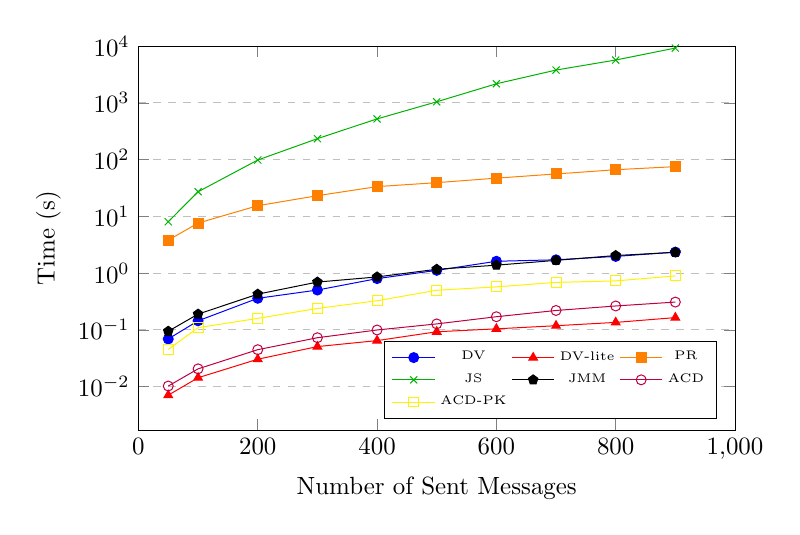
\begin{tikzpicture}[scale=0.9]
\begin{axis}[
  ymode=log,
 legend style={font=\tiny, legend columns=3},
  scaled ticks=false,
  xlabel={Number of Sent Messages},
  ylabel={Time (s)},
  xmin=0, xmax=1000,
  ymax=10000,
  xtick={0,200,400,600,800,1000},
  ytick={0.01,0.1,1,10,100,1000,10000},
  legend pos=south east,
  ymajorgrids=true,
  xminorticks=false,
  yminorticks=false,
  grid style=dashed,
  height=7cm,
  width=10cm,
]
 
\addplot[color=blue,mark=*]
   coordinates {
  (50,0.0689)(100,0.144)(200,0.359)(300,0.502)(400,0.798)(500,1.116)(600,1.614)
  (700,1.712)(800,1.965)(900,2.344)
  };

\addplot[color=red,mark=triangle*]
  coordinates {
  (50,0.00704)(100,0.0143)(200,0.0303)(300,0.0506)(400,0.0645)(500,0.0923)
  (600,0.104)(700,0.118)(800,0.135)(900,0.164)
  };

\addplot[color=orange,mark=square*]
  coordinates {
  (50,3.8)(100,7.6)(200,15.4)(300,23.1)(400,33.4)(500,39.2)
  (600,47.1)(700,55.8)(800,66.3)(900,75.1)
  };

\addplot[color=black!30!green,mark=x]
  coordinates {
  (50,8.024)(100,27.096)(200,98.210)(300,233.751)(400,521.110)(500,1044.091)
  (600,2168.099)(700,3783.724)(800,5688.493)(900,9235.921)
  };

\addplot[color=black,mark=pentagon*]
  coordinates {
  (50,0.0943)(100,0.189)(200,0.425)(300,0.694)(400,0.854)(500,1.166)
  (600,1.377)(700,1.675)(800,2.036)(900,2.319)
  };

\addplot[color=purple,mark=o]
  coordinates {
  (50,0.0102)(100,0.0205)(200,0.0446)(300,0.0725)(400,0.0992)(500,0.127)
  (600,0.170)(700,0.219)(800,0.263)(900,0.308)
  };

\addplot[color=yellow,mark=square]
  coordinates {
  (50,0.0451)(100,0.109)(200,0.159)(300,0.238)(400,0.325)(500,0.498)
  (600,0.571)(700,0.685)(800,0.727)(900,0.891)
  };

  \legend{DV,DV-lite,PR,JS,JMM,ACD,ACD-PK}
 
\end{axis}
\end{tikzpicture} 
  \end{figure}
\end{frame}

\begin{frame}{Runtime (Unidirectional) II.}
  \scriptsize
  \begin{table}
    \caption*{PR (Poettering \& Rösler)}
    \begin{tabular}{ | l | l | l | l |}
    \hline
    Primitive & Generations & (Encs/Decs) $\vee$ (Sigs/Vers) & Updates PK/SK \\ \hline
    \textbf{ku-KEM} & $2n$ & $\frac{3}{2}n/\frac{3}{2}n$ & $0/0$ \\ \hline
    \textbf{Signature} & $n$ & $n/n$ & - \\  
    \hline
    \end{tabular}
  \end{table}
  \begin{table}
    \caption*{JS (Jaeger \& Stepanovs)}
    \begin{tabular}{ | l | l | l | l |}
    \hline
    Primitive & Generations & (Encs/Decs) $\vee$ (Sigs/Vers) & Updates PK/SK \\ \hline
    \textbf{ku-PKE} & $n$ & $n/n$ & $\frac{(n-1)n}{2}/n$ \\ \hline
    \textbf{ku-Sig} & $n$ & $n/n$ & $\frac{n}{2}/n$ \\  
    \hline
    \end{tabular}
  \end{table}
\end{frame}

\begin{frame}{Runtime (Unidirectional) III.}
  \scriptsize
  \begin{table}
    \caption*{DV (Durak \& Vaudenay)}
    \begin{tabular}{ | l | l | l | l |}
    \hline
    Primitive & Generations & (Encs/Decs) $\vee$ (Sigs/Vers) & Updates PK/SK \\ \hline
    \textbf{PKE} & $2n$ & $\frac{3}{2}n/\frac{3}{2}n$ & $0/0$ \\ \hline
    \textbf{Signature} & $2n$ & $\frac{3}{2}n/\frac{3}{2}n$ & $0/0$ \\  
    \hline
    \end{tabular}
  \end{table}
  \begin{table}
    \caption*{JMM (Jost, Maurer \& Mularczyk)}
    \begin{tabular}{ | l | l | l | l |}
    \hline
    Primitive & Generations & (Encs/Decs) $\vee$ (Sigs/Vers) & Updates PK/SK \\ \hline
    \textbf{Sig} & $2n$ & $n/n$ & - \\ \hline
    \textbf{ku-Sig} & $0$ & $n/n$ & - \\ \hline
    \textbf{sku-PKE} & $2n$ & $n/n$ & $n/n$ \\ \hline
    \textbf{PKE-AD} & $3n$ & $n/n$ & - \\
    \hline
    \end{tabular}
  \end{table}
\end{frame}

\begin{frame}{Runtime (Unidirectional) IV.}
  \scriptsize
  \begin{table}
    \caption*{ACD (Alwen, Coretti \& Dodis)}
    \begin{tabular}{ | l | l | l | l |}
    \hline
    Primitive & Generations & (Encs/Decs) $\vee$ (Sigs/Vers) & Updates PK/SK \\ \hline
    \textbf{FS-AEAD} & $4$ & $n/n$ & - \\ \hline
    \textbf{CKA} & $4$ & - & - \\  
    \hline
    \end{tabular}
  \end{table}
  \normalsize
  \begin{itemize}
  \item Quadratic key-update penalty for the JS protocol.
  \item Other protocols either slightly faster or unchanged.
  \end{itemize}
\end{frame}

\begin{frame}{Runtime (Deferred Unidirectional) I.}
 \begin{figure}[H]
    \centering
    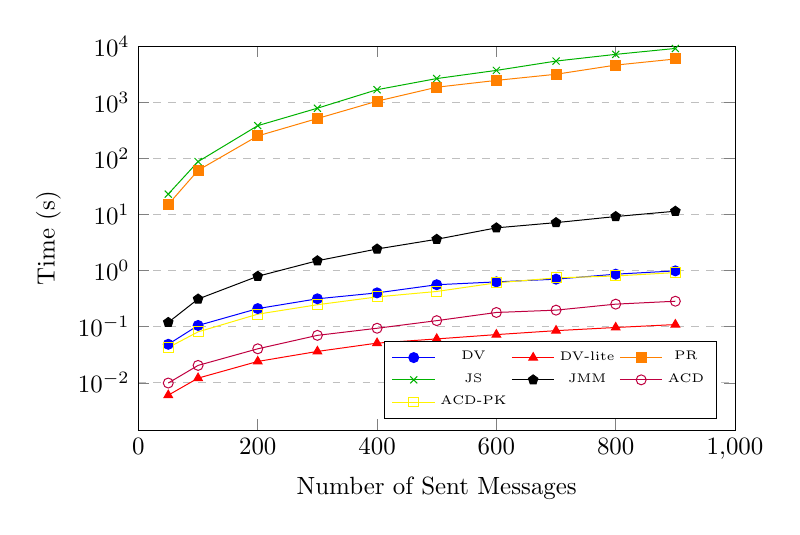
\begin{tikzpicture}[scale=0.9]
\begin{axis}[
  ymode=log,
  legend style={font=\tiny, legend columns=3},
  scaled ticks=false,
  xlabel={Number of Sent Messages},
  ylabel={Time (s)},
  xmin=0, xmax=1000,
  ymax=10000,
  xtick={0,200,400,600,800,1000},
  ytick={0.01,0.1,1,10,100,1000,10000},
  legend pos=south east,
  ymajorgrids=true,
  xminorticks=false,
  yminorticks=false,
  grid style=dashed,
  height=7cm,
  width=10cm,
]
 
\addplot[color=blue,mark=*]
   coordinates {
  (50,0.0485)(100,0.105)(200,0.210)(300,0.314)(400,0.400)(500,0.559)(600,0.628)
  (700,0.702)(800,0.862)(900,0.987)
  };

\addplot[color=red,mark=triangle*]
  coordinates {
  (50,0.00601)(100,0.0121)(200,0.0240)(300,0.0362)(400,0.0509)(500,0.0605)
  (600,0.0722)(700,0.0849)(800,0.0967)(900,0.109)
  };

\addplot[color=orange,mark=square*]
  coordinates {
  (50,15.052)(100,61.132)(200,250.773)(300,512.437)(400,1043.941)(500,1849.874)
  (600,2449.326)(700,3149.923)(800,4587.110)(900,5897.349)
  };


\addplot[color=black!30!green,mark=x]
  coordinates {
  (50,23.084)(100,87.370)(200,382.419)(300,782.271)(400,1672.800)(500,2640.221)
  (600,3691.952)(700,5413.382)(800,7129.012)(900,9087.283)
  };

\addplot[color=black,mark=pentagon*]
  coordinates {
  (50,0.119)(100,0.311)(200,0.791)(300,1.496)(400,2.421)(500,3.608)
  (600,5.770)(700,7.148)(800,9.172)(900,11.411)
  };

\addplot[color=purple,mark=o]
  coordinates {
  (50,0.0099)(100,0.0204)(200,0.0403)(300,0.0700)(400,0.0937)(500,0.128)
  (600,0.179)(700,0.197)(800,0.252)(900,0.284)
  };

\addplot[color=yellow,mark=square]
  coordinates {
  (50,0.0424)(100,0.0808)(200,0.167)(300,0.246)(400,0.339)(500,0.424)
  (600,0.604)(700,0.740)(800,0.801)(900,0.920)
  };

    
  \legend{DV,DV-lite,PR,JS,JMM,ACD,ACD-PK}
 
\end{axis}
\end{tikzpicture} 
  \end{figure}
\end{frame}

\begin{frame}{Runtime (Deferred Unidirectional) II.}
  \scriptsize
  \begin{table}
    \caption*{PR (Poettering \& Rösler)}
    \begin{tabular}{ | l | l | l | l |}
    \hline
    Primitive & Generations & (Encs/Decs) $\vee$ (Sigs/Vers) & Updates PK/SK \\ \hline
    \textbf{ku-KEM} & $2n$ & $n/n$ & $2(\frac{n}{2})^2/2(\frac{n}{2})^2$ \\ \hline
    \textbf{Signature} & $n$ & $n/n$ & - \\  
    \hline
    \end{tabular}
  \end{table}
  \begin{table}
    \caption*{JS (Jaeger \& Stepanovs)}
    \begin{tabular}{ | l | l | l | l |}
    \hline
    Primitive & Generations & (Encs/Decs) $\vee$ (Sigs/Vers) & Updates PK/SK \\ \hline
    \textbf{ku-PKE} & $n$ & $n/n$ & $\frac{(n-1)n}{2}/n(\frac{n}{2}+1)$ \\ \hline
    \textbf{ku-Sig} & $n$ & $n/n$ & $0/n$ \\  
    \hline
    \end{tabular}
  \end{table}
\end{frame}

\begin{frame}{Runtime (Deferred Unidirectional) III.}
  \scriptsize
  \begin{table}
    \caption*{DV (Durak \& Vaudenay)}
    \begin{tabular}{ | l | l | l | l |}
    \hline
    Primitive & Generations & (Encs/Decs) $\vee$ (Sigs/Vers) & Updates PK/SK \\ \hline
    \textbf{PKE} & $2n$ & $n/n$ & $0/0$ \\ \hline
    \textbf{Signature} & $2n$ & $n/n$ & $0/0$ \\  
    \hline
    \end{tabular}
  \end{table}
  \begin{table}
    \caption*{JMM (Jost, Maurer \& Mularczyk)}
    \begin{tabular}{ | l | l | l | l |}
    \hline
    Primitive & Generations & (Encs/Decs) $\vee$ (Sigs/Vers) & Updates PK/SK \\ \hline
    \textbf{Sig} & $2n$ & $n/n$ & - \\ \hline
    \textbf{ku-Sig} & $0$ & $n/n$ & - \\ \hline
    \textbf{sku-PKE} & $2n$ & $n/n$ & $n+2n^2/n+2n^2$ \\ \hline
    \textbf{PKE-AD} & $3n$ & $n/n$ & - \\
    \hline
    \end{tabular}
  \end{table}
\end{frame}

\begin{frame}{Runtime (Deferred Unidirectional) IV.}
  \scriptsize
  \begin{table}
    \caption*{ACD (Alwen, Coretti \& Dodis)}
    \begin{tabular}{ | l | l | l | l |}
    \hline
    Primitive & Generations & (Encs/Decs) $\vee$ (Sigs/Vers) & Updates PK/SK \\ \hline
    \textbf{FS-AEAD} & $2$ & $n/n$ & - \\ \hline
    \textbf{CKA} & $2$ & - & - \\  
    \hline
    \end{tabular}
  \end{table}
  \normalsize
  \begin{itemize}
  \item Now also quadratic key-update penalties for the PR and JMM protocols.
  \item Clear separation between the DV and JMM protocols.
  \end{itemize}
\end{frame}

\begin{frame}{Message Size (Alternating)}
   \begin{figure}[H]
    \centering
    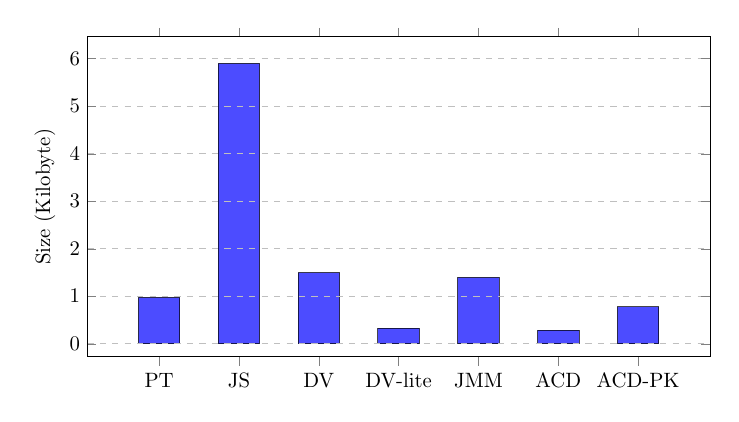
\begin{tikzpicture}[scale=.75]
  \begin{axis} [
    ybar, axis on top,
    bar width= 20pt,
    legend pos=north west,
    ylabel={Size (Kilobyte)},
    symbolic x coords={PT,JS,DV, DV-lite, JMM, ACD, ACD-PK},
    xtick=data,
    ytick={0,1,2,3,4,5,6},
    nodes near coords={},
    grid style=dashed,
    ymajorgrids=true,
    yminorticks=false,
    xminorticks=false,
    legend style={at={(0.5,1)},
    anchor=north,legend columns=-1},
    %xticklabel style = {rotate=75},
    height=7cm,
    width=\textwidth,
    enlarge x limits=0.15,
  ]

   y=-0.5cm,      \addplot [
      fill=blue,
      opacity=0.7,
      area legend,
    ] coordinates {
        (PT,0.98)
        (JS,5.9)
        (DV,1.5)
	(DV-lite,0.33)
        (JMM,1.4)
        (ACD,0.29)
        (ACD-PK,0.78)
    };

%    \addplot [
%      fill=purple,
%      opacity=0.7,
%      area legend,
%    ] coordinates {
%        (Alternating,3260.4) +- (0,47.432291)
%        (Unidirectional,6148.4) +- (0,112.415104)
%        (Def. Unidirectional,10852.9) +- (0,43.195807)
%    };
%    
%    \addplot [
%      fill=red,
%      opacity=0.7,
%      area legend,
%    ] coordinates {
%        (Alternating,33459.41112) +- (0,592.258861)
%        (Unidirectional,64690.703011) +- (0,1429.674333)
%        (Def. Unidirectional,131962.165976) +- (0,911.453089)
%    };
%
%   \addplot [
%      fill=red,
%      opacity=0.7,
%      area legend,
%    ] coordinates {
%        (Alternating,33459.41112) +- (0,592.258861)
%        (Unidirectional,64690.703011) +- (0,1429.674333)
%        (Def. Unidirectional,131962.165976) +- (0,911.453089)
%    };
%
%       \addplot [
%      fill=orange,
%      opacity=0.7,
%      area legend,
%    ] coordinates {
%        (Alternating,33459.41112) +- (0,592.258861)
%        (Unidirectional,64690.703011) +- (0,1429.674333)
%        (Def. Unidirectional,131962.165976) +- (0,911.453089)
%    };
%
%       \addplot [
%      fill=yellow,
%      opacity=0.7,
%      area legend,
%    ] coordinates {
%        (Alternating,33459.41112) +- (0,592.258861)
%        (Unidirectional,64690.703011) +- (0,1429.674333)
%        (Def. Unidirectional,131962.165976) +- (0,911.453089)
%    };
%
%     \addplot [
%      fill=green,
%      opacity=0.7,
%      area legend,
%    ] coordinates {
%        (Alternating,33459.41112) +- (0,592.258861)
%        (Unidirectional,64690.703011) +- (0,1429.674333)
%        (Def. Unidirectional,131962.165976) +- (0,911.453089)
%    };

%    \legend{PR, JS, DV, DV-lite, JMM, ACD, ACD-PK}
  \end{axis}
\end{tikzpicture} 
  \end{figure}
\end{frame}

\begin{frame}{Message Size (Unidirectional)}
   \begin{figure}[H]
    \centering
    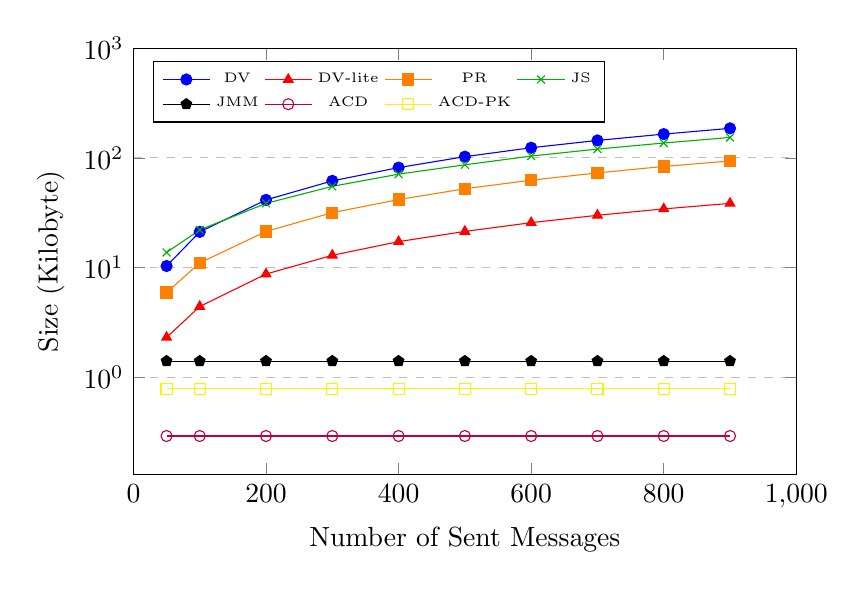
\begin{tikzpicture}[scale=1]
\begin{axis}[
  %ymode=log,
%  legend style={font=\tiny, legend columns=4},
%  scaled ticks=false,
%  xlabel={Number of Sent Messages},
%  ylabel={Size (Kilobyte)},
%  xmin=0, xmax=1000,
%  ymax=200,
%  xtick={0,200,400,600,800,1000},
%  %ytick={0.01,0.1,1,10,100,1000,10000},
%  ytick={0,20,40,60,80,100,120,140,160,180,200},
%  legend pos=north west,
%  ymajorgrids=true,
%  xminorticks=false,
%  yminorticks=false,
%  grid style=dashed,
%  height=7cm,
%  width=10cm,
  ymode=log,
  legend style={font=\tiny, legend columns=4},
  scaled ticks=false,
  xlabel={Number of Sent Messages},
  ylabel={Size (Kilobyte)},
  xmin=0, xmax=1000,
  ymax=1000,
  xtick={0,200,400,600,800,1000},
  ytick={0.001,0.01,0.1,1,10,100,1000},
  %ytick={0,20,40,60,80,100,120,140,160,180,200},
  legend pos=north west,
  ymajorgrids=true,
  xminorticks=false,
  yminorticks=false,
  grid style=dashed,
  height=7cm,
  width=10cm,
]
 
\addplot[color=blue,mark=*]
   coordinates {
  (50,10.3)(100,21.1)(200,41.3)(300,61.6)(400,81.4)(500,102.4)(600,123.5)
  (700,144.0)(800,164.5)(900,185.6)
  };

\addplot[color=red,mark=triangle*]
  coordinates {
  (50,2.3)(100,4.4)(200,8.7)(300,12.9)(400,17.2)(500,21.3)
  (600,25.6)(700,29.9)(800,34.2)(900,38.4)
  };

\addplot[color=orange,mark=square*]
  coordinates {
  (50,5.9)(100,11.0)(200,21.3)(300,31.6)(400,41.6)(500,52.2)
  (600,62.5)(700,72.8)(800,83.4)(900,93.5)
  };


\addplot[color=black!30!green,mark=x]
  coordinates {
  (50,13.7)(100,22.0)(200,38.4)(300,54.9)(400,70.9)(500,86.3)
  (600,103.7)(700,120.1)(800,136.4)(900,153.3)
  };

\addplot[color=black,mark=pentagon*]
  coordinates {
  (50,1.4)(100,1.4)(200,1.4)(300,1.4)(400,1.4)(500,1.4)
  (600,1.4)(700,1.4)(800,1.4)(900,1.4)
  };

\addplot[color=purple,mark=o]
  coordinates {
  (50,0.29)(100,0.29)(200,0.29)(300,0.29)(400,0.29)(500,0.29)
  (600,0.29)(700,0.29)(800,0.29)(900,0.29)
  };

\addplot[color=yellow,mark=square]
  coordinates {
  (50,0.78)(100,0.78)(200,0.78)(300,0.78)(400,0.78)(500,0.78)
  (600,0.78)(700,0.78)(800,0.78)(900,0.78)
  };


  \legend{DV,DV-lite,PR,JS,JMM,ACD,ACD-PK}
 
\end{axis}
\end{tikzpicture} 
  \end{figure}
\end{frame}

\begin{frame}{Message Size (Deferred Unidirectional)}
   \begin{figure}[H]
    \centering
    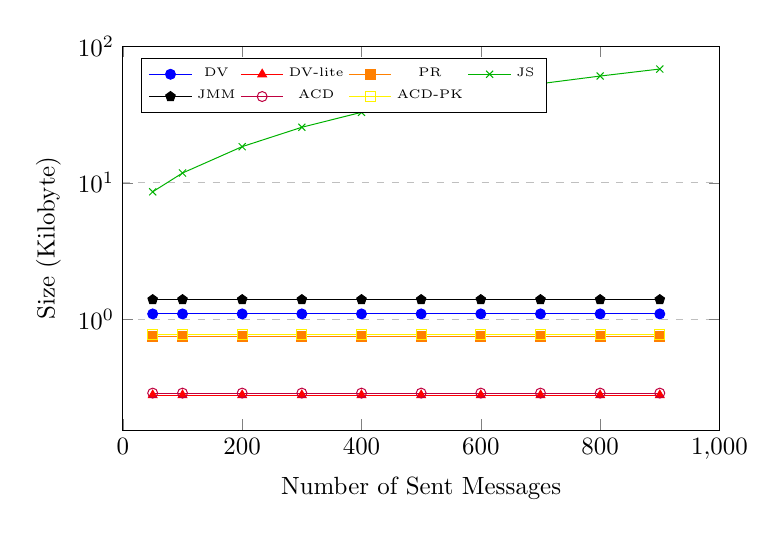
\begin{tikzpicture}[scale=0.9]
\begin{axis}[
  ymode=log,
  legend style={font=\tiny, legend columns=4},
  scaled ticks=false,
  xlabel={Number of Sent Messages},
  ylabel={Size (Kilobyte)},
  xmin=0, xmax=1000,
  ymax=100,
  xtick={0,200,400,600,800,1000},
  ytick={0.001,0.01,0.1,1,10,100},
  %ytick={0,20,40,60,80,100,120,140,160,180,200},
  legend pos=north west,
  ymajorgrids=true,
  xminorticks=false,
  yminorticks=false,
  grid style=dashed,
  height=7cm,
  width=10cm,
]
 
\addplot[color=blue,mark=*]
   coordinates {
  (50,1.1)(100,1.1)(200,1.1)(300,1.1)(400,1.1)(500,1.1)(600,1.1)
  (700,1.1)(800,1.1)(900,1.1)
  };

\addplot[color=red,mark=triangle*]
  coordinates {
  (50,0.28)(100,0.28)(200,0.28)(300,0.28)(400,0.28)(500,0.28)
  (600,0.28)(700,0.28)(800,0.28)(900,0.28)
  };

\addplot[color=orange,mark=square*]
  coordinates {
  (50,0.75)(100,0.75)(200,0.75)(300,0.75)(400,0.75)(500,0.75)
  (600,0.75)(700,0.75)(800,0.75)(900,0.75)
  };

\addplot[color=black!30!green,mark=x]
  coordinates {
  (50,8.6)(100,11.8)(200,18.4)(300,25.5)(400,32.8)(500,39.9)
  (600,46.3)(700,53.1)(800,60.4)(900,68.0)
  };

\addplot[color=black,mark=pentagon*]
  coordinates {
  (50,1.4)(100,1.4)(200,1.4)(300,1.4)(400,1.4)(500,1.4)
  (600,1.4)(700,1.4)(800,1.4)(900,1.4)
  };

\addplot[color=purple,mark=o]
  coordinates {
  (50,0.29)(100,0.29)(200,0.29)(300,0.29)(400,0.29)(500,0.29)
  (600,0.29)(700,0.29)(800,0.29)(900,0.29)
  };

\addplot[color=yellow,mark=square]
  coordinates {
  (50,0.78)(100,0.78)(200,0.78)(300,0.78)(400,0.78)(500,0.78)
  (600,0.78)(700,0.78)(800,0.78)(900,0.78)
  };

  \legend{DV,DV-lite,PR,JS,JMM,ACD,ACD-PK}
 
\end{axis}
\end{tikzpicture} 
  \end{figure}
\end{frame}

\begin{frame}{State Size (Alternating)}
   \begin{figure}[H]
    \centering
    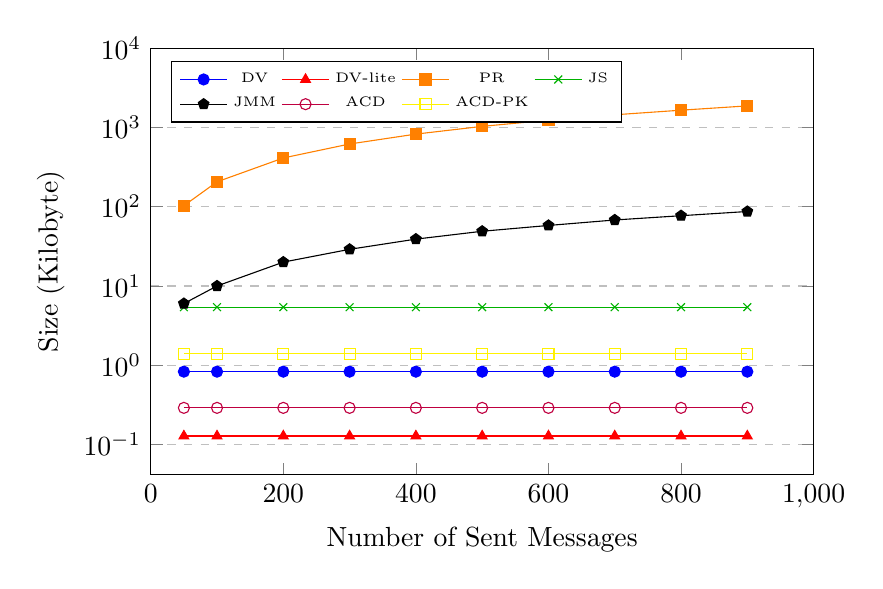
\begin{tikzpicture}[scale=1]
\begin{axis}[
  %ymode=log,
%  legend style={font=\tiny, legend columns=4},
%  scaled ticks=false,
%  xlabel={Number of Sent Messages},
%  ylabel={Size (Kilobyte)},
%  xmin=0, xmax=1000,
%  ymax=200,
%  xtick={0,200,400,600,800,1000},
%  %ytick={0.01,0.1,1,10,100,1000,10000},
%  ytick={0,20,40,60,80,100,120,140,160,180,200},
%  legend pos=north west,
%  ymajorgrids=true,
%  xminorticks=false,
%  yminorticks=false,
%  grid style=dashed,
%  height=7cm,
%  width=10cm,
  ymode=log,
  legend style={font=\tiny, legend columns=4},
  scaled ticks=false,
  xlabel={Number of Sent Messages},
  ylabel={Size (Kilobyte)},
  xmin=0, xmax=1000,
  ymax=10000,
  xtick={0,200,400,600,800,1000},
  ytick={0.001,0.01,0.1,1,10,100,1000,10000},
  %ytick={0,20,40,60,80,100,120,140,160,180,200},
  legend pos=north west,
  ymajorgrids=true,
  xminorticks=false,
  yminorticks=false,
  grid style=dashed,
  height=7cm,
  width=10cm,
]
 
\addplot[color=blue,mark=*]
   coordinates {
  (50,0.83)(100,0.83)(200,0.83)(300,0.83)(400,0.83)(500,0.83)(600,0.83)
  (700,0.83)(800,0.83)(900,0.83)
  };

\addplot[color=red,mark=triangle*]
  coordinates {
  (50,0.128)(100,0.128)(200,0.128)(300,0.128)(400,0.128)(500,0.128)
  (600,0.128)(700,0.128)(800,0.128)(900,0.128)
  };

\addplot[color=orange,mark=square*]
  coordinates {
  (50,103)(100,206)(200,412)(300,618)(400,824)(500,1031)
  (600,1237)(700,1444)(800,1650)(900,1870)
  };


\addplot[color=black!30!green,mark=x]
  coordinates {
  (50,5.4)(100,5.4)(200,5.4)(300,5.4)(400,5.4)(500,5.4)
  (600,5.4)(700,5.4)(800,5.4)(900,5.4)
  };

\addplot[color=black,mark=pentagon*]
  coordinates {
  (50,6)(100,10)(200,20)(300,29)(400,39)(500,49)
  (600,58)(700,68)(800,77)(900,87)
  };

\addplot[color=purple,mark=o]
  coordinates {
  (50,0.29)(100,0.29)(200,0.29)(300,0.29)(400,0.29)(500,0.29)
  (600,0.29)(700,0.29)(800,0.29)(900,0.29)
  };

\addplot[color=yellow,mark=square]
  coordinates {
  (50,1.4)(100,1.4)(200,1.4)(300,1.4)(400,1.4)(500,1.4)
  (600,1.4)(700,1.4)(800,1.4)(900,1.4)
  };


  \legend{DV,DV-lite,PR,JS,JMM,ACD,ACD-PK}
 
\end{axis}
\end{tikzpicture} 
  \end{figure}
\end{frame}

\begin{frame}{State Size ([Deferred] Unidirectional)}
   \begin{figure}[H]
    \centering
    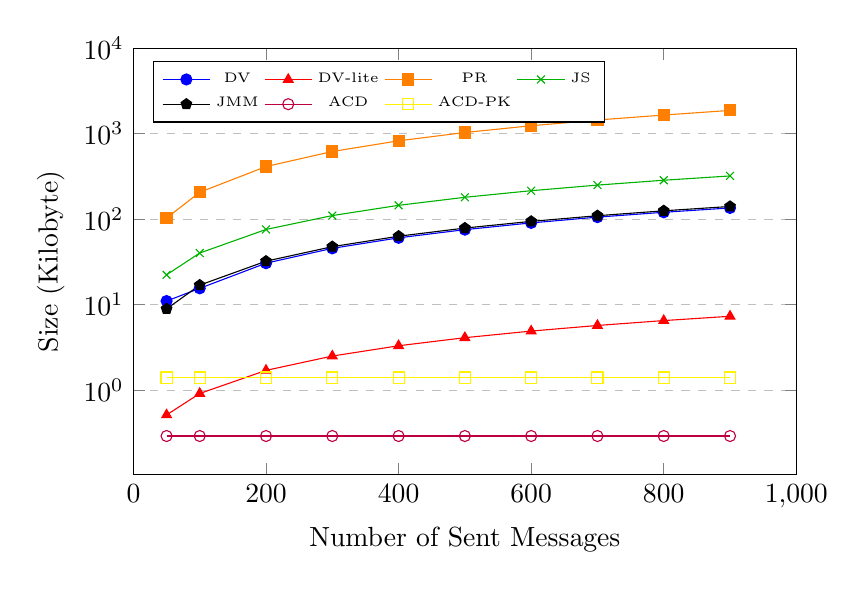
\begin{tikzpicture}[scale=1]
\begin{axis}[
  %ymode=log,
%  legend style={font=\tiny, legend columns=4},
%  scaled ticks=false,
%  xlabel={Number of Sent Messages},
%  ylabel={Size (Kilobyte)},
%  xmin=0, xmax=1000,
%  ymax=200,
%  xtick={0,200,400,600,800,1000},
%  %ytick={0.01,0.1,1,10,100,1000,10000},
%  ytick={0,20,40,60,80,100,120,140,160,180,200},
%  legend pos=north west,
%  ymajorgrids=true,
%  xminorticks=false,
%  yminorticks=false,
%  grid style=dashed,
%  height=7cm,
%  width=10cm,
  ymode=log,
  legend style={font=\tiny, legend columns=4},
  scaled ticks=false,
  xlabel={Number of Sent Messages},
  ylabel={Size (Kilobyte)},
  xmin=0, xmax=1000,
  ymax=10000,
  xtick={0,200,400,600,800,1000},
  ytick={0.001,0.01,0.1,1,10,100,1000,10000},
  %ytick={0,20,40,60,80,100,120,140,160,180,200},
  legend pos=north west,
  ymajorgrids=true,
  xminorticks=false,
  yminorticks=false,
  grid style=dashed,
  height=7cm,
  width=10cm,
]
 
\addplot[color=blue,mark=*]
   coordinates {
  (50,11.0)(100,15.5)(200,30.5)(300,45.5)(400,60.4)(500,75.3)(600,90.3)
  (700,105.5)(800,120.2)(900,135.1)
  };

\addplot[color=red,mark=triangle*]
  coordinates {
  (50,0.512)(100,0.912)(200,1.7)(300,2.5)(400,3.3)(500,4.1)
  (600,4.9)(700,5.7)(800,6.5)(900,7.3)
  };

\addplot[color=orange,mark=square*]
  coordinates {
  (50,103)(100,206)(200,412)(300,618)(400,824)(500,1031)
  (600,1237)(700,1444)(800,1650)(900,1870)
  };


\addplot[color=black!30!green,mark=x]
  coordinates {
  (50,22.3)(100,40.1)(200,75.7)(300,110)(400,145)(500,180)
  (600,215)(700,250)(800,285)(900,320)
  };

\addplot[color=black,mark=pentagon*]
  coordinates {
  (50,8.9)(100,16.9)(200,32.2)(300,47.6)(400,63.1)(500,78.6)
  (600,94.1)(700,109.6)(800,125.1)(900,140.6)
  };

\addplot[color=purple,mark=o]
  coordinates {
  (50,0.29)(100,0.29)(200,0.29)(300,0.29)(400,0.29)(500,0.29)
  (600,0.29)(700,0.29)(800,0.29)(900,0.29)
  };

\addplot[color=yellow,mark=square]
  coordinates {
  (50,1.4)(100,1.4)(200,1.4)(300,1.4)(400,1.4)(500,1.4)
  (600,1.4)(700,1.4)(800,1.4)(900,1.4)
  };


  \legend{DV,DV-lite,PR,JS,JMM,ACD,ACD-PK}
 
\end{axis}
\end{tikzpicture} 
  \end{figure}
\end{frame}

\section{Erratum}
\label{sec:erratum}



\section{Conclusion}
\label{sec:conclusion}

\begin{frame}{Future Work}
  
\end{frame}

\begin{frame}{Gained Knowledge}
  
\end{frame}

\end{document}
